\chapter*{Les îles Galapagos\markboth{Les îles Galapagos}{}}
\section*{14 juillet 2015}

3h d'avion depuis Quito pour arriver sur l'île de Baltra. Une courte traversée et 1h de bus mènent à Puerto Ayora, la ville principale de l'île Santa Cruz. 
\begin{center} 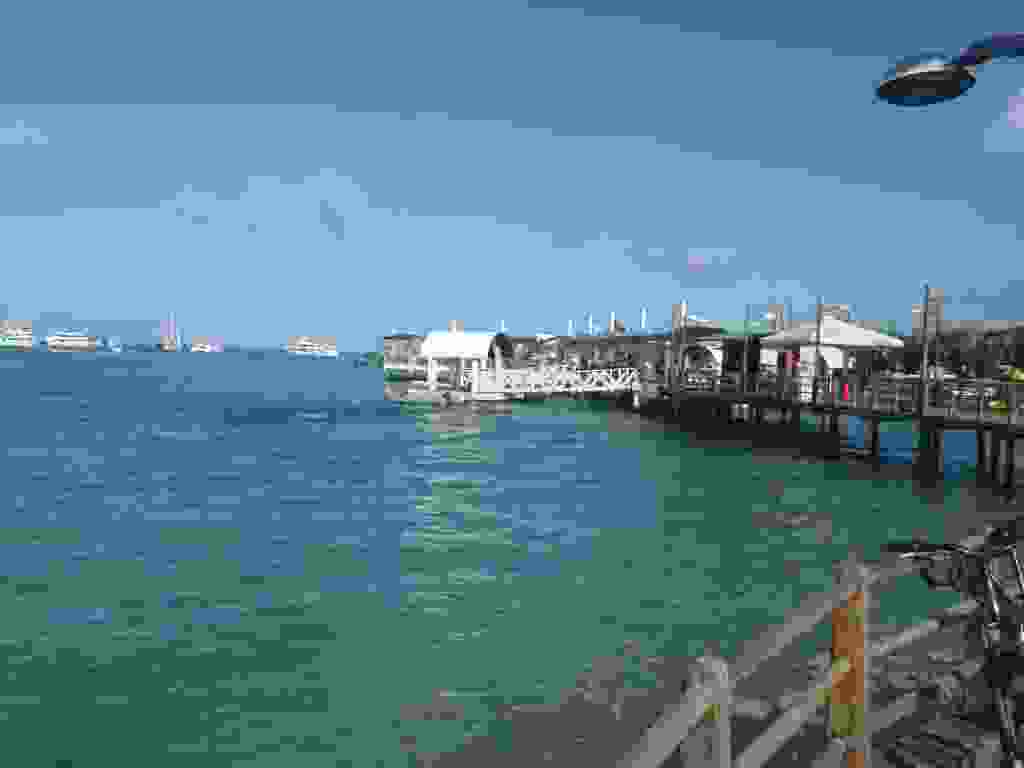
\includegraphics[width=\mywidth]{../wp-content/uploads/2015/07/P7015189-1024x768.jpg} \end{center}
\begin{center} 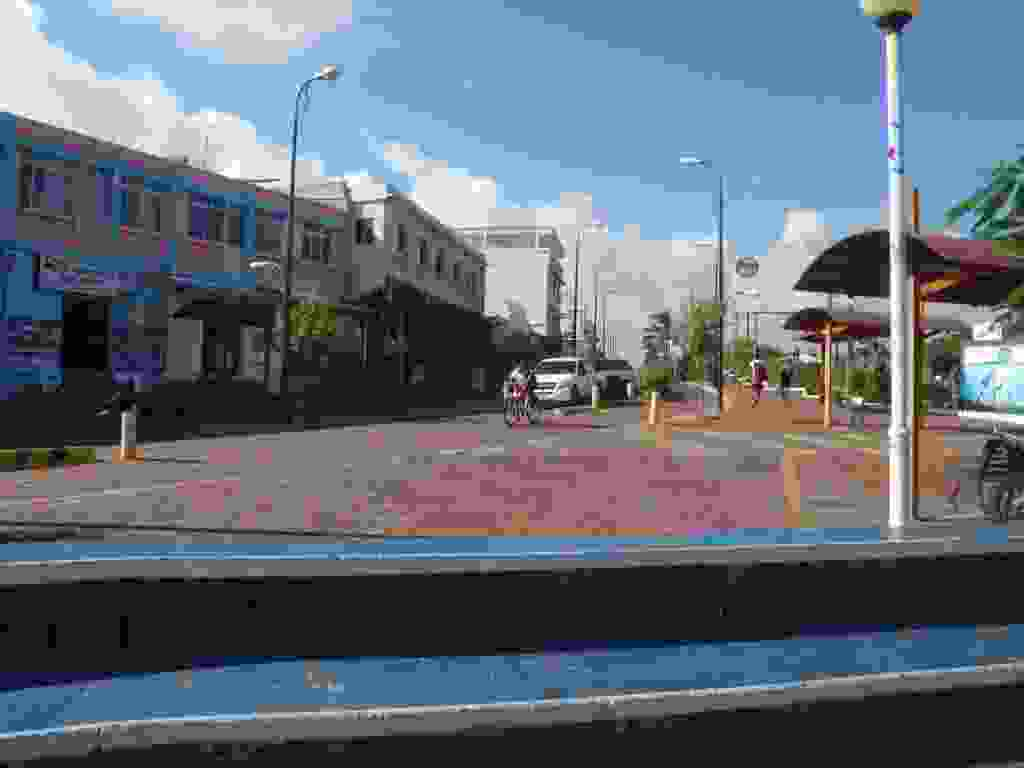
\includegraphics[width=\mywidth]{../wp-content/uploads/2015/07/P7015191-1024x768.jpg} \end{center}

Je visite le centre Charles Darwin où on peut observer des tortues et des iguanes. 
\begin{center} 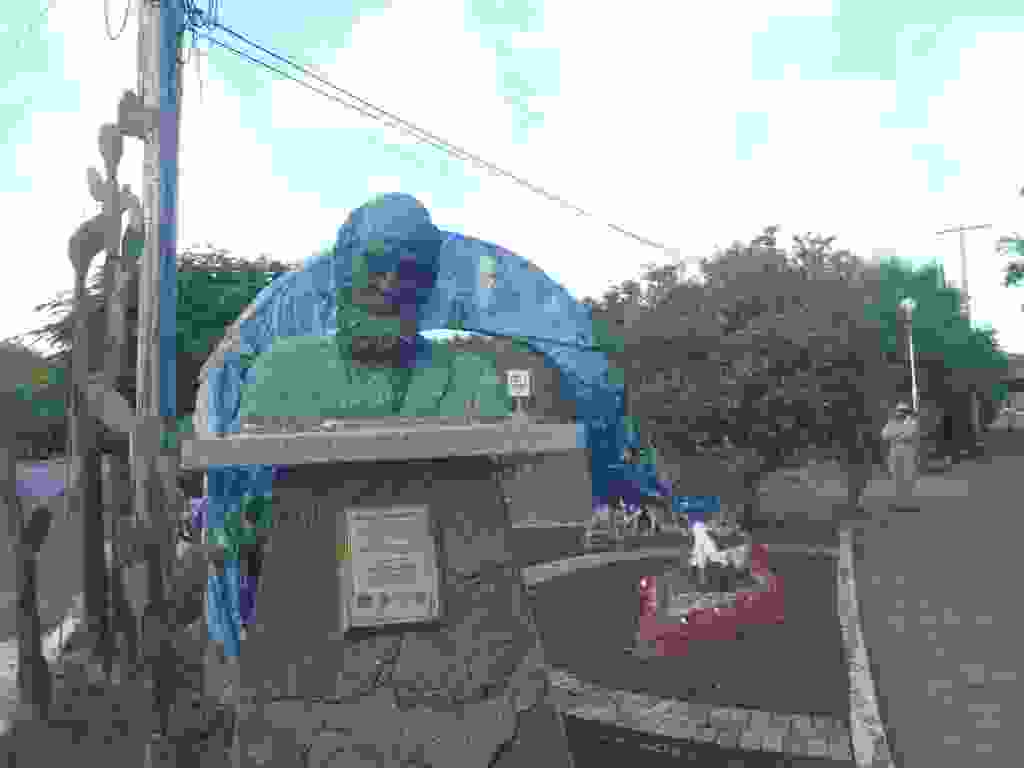
\includegraphics[width=\mywidth]{../wp-content/uploads/2015/07/P7025192-1024x768.jpg} \end{center}
\begin{center} 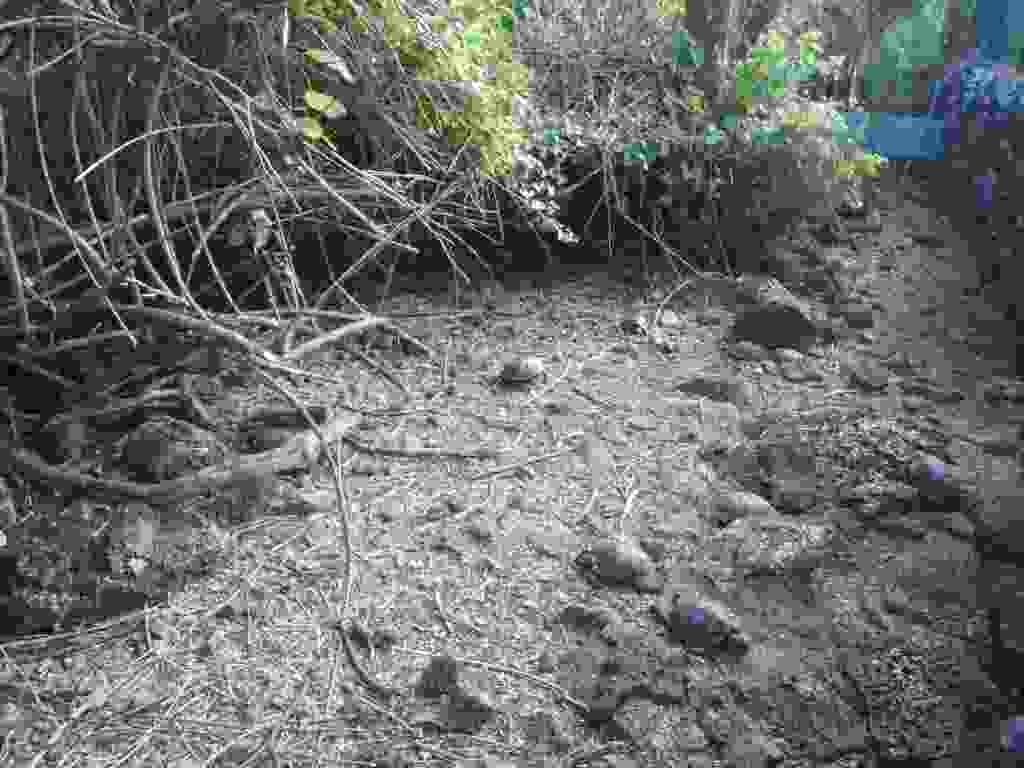
\includegraphics[width=\mywidth]{../wp-content/uploads/2015/07/P7025196-1024x768.jpg} \end{center}
\begin{center} 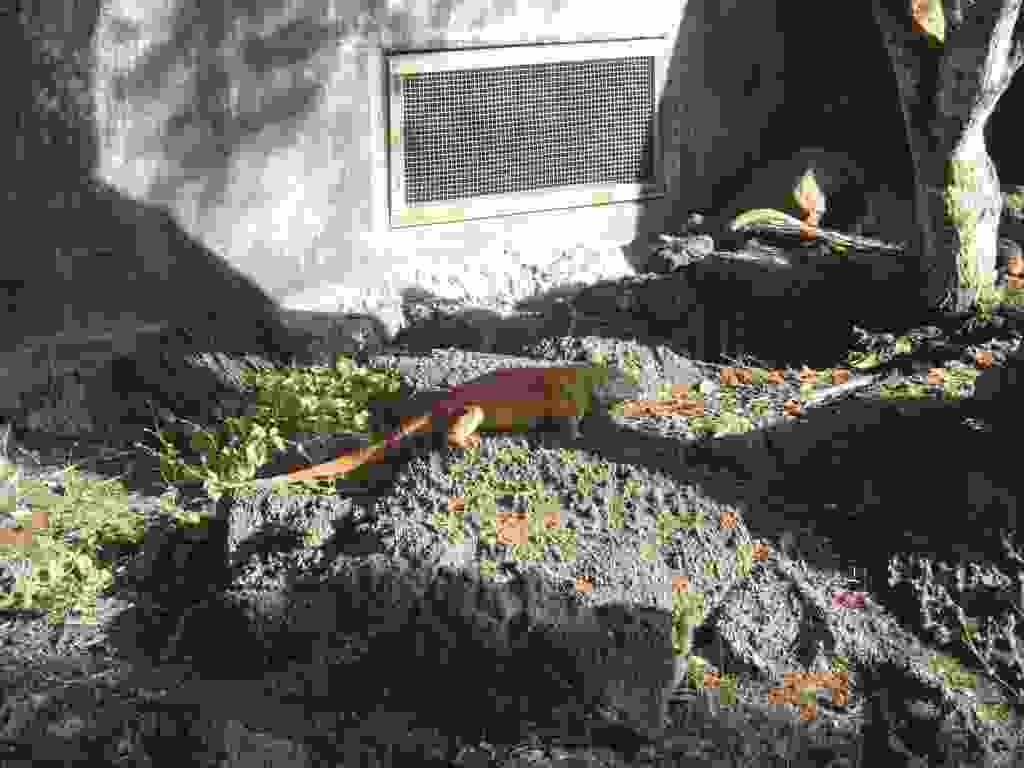
\includegraphics[width=\mywidth]{../wp-content/uploads/2015/07/P7025200-1024x768.jpg} \end{center}
\begin{center} 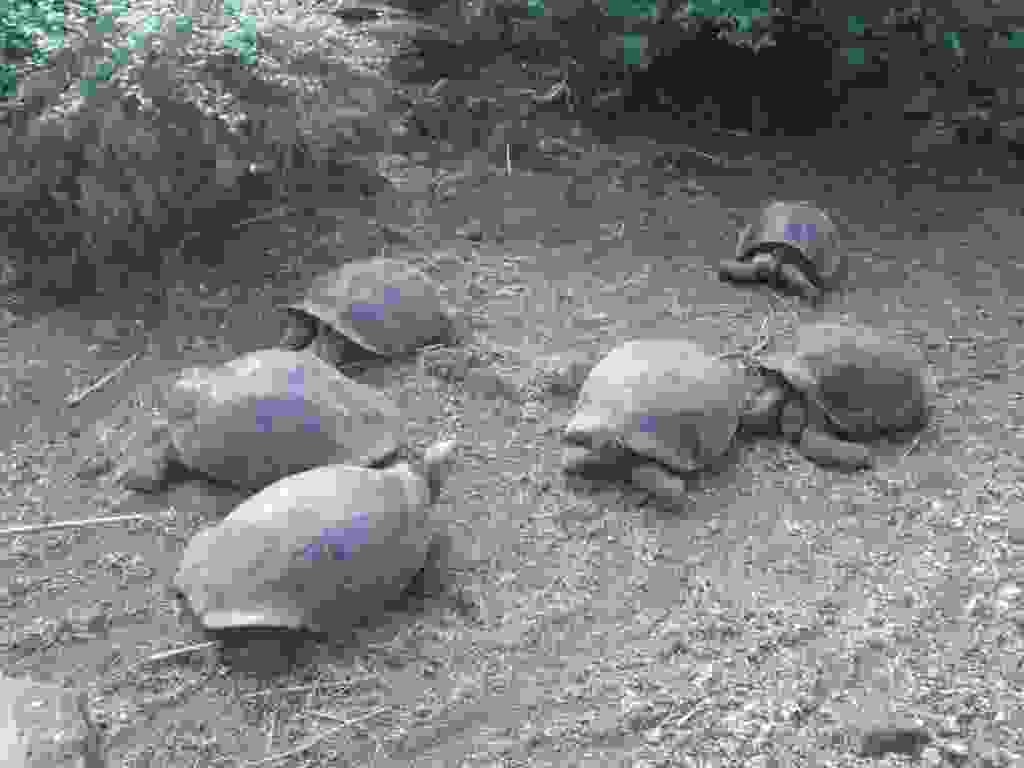
\includegraphics[width=\mywidth]{../wp-content/uploads/2015/07/P7025204-1024x768.jpg} \end{center}

Je me rends en stop à la réserve d'El Chato au centre de l'île. Les tortues sont ici en liberté. 
\begin{center} 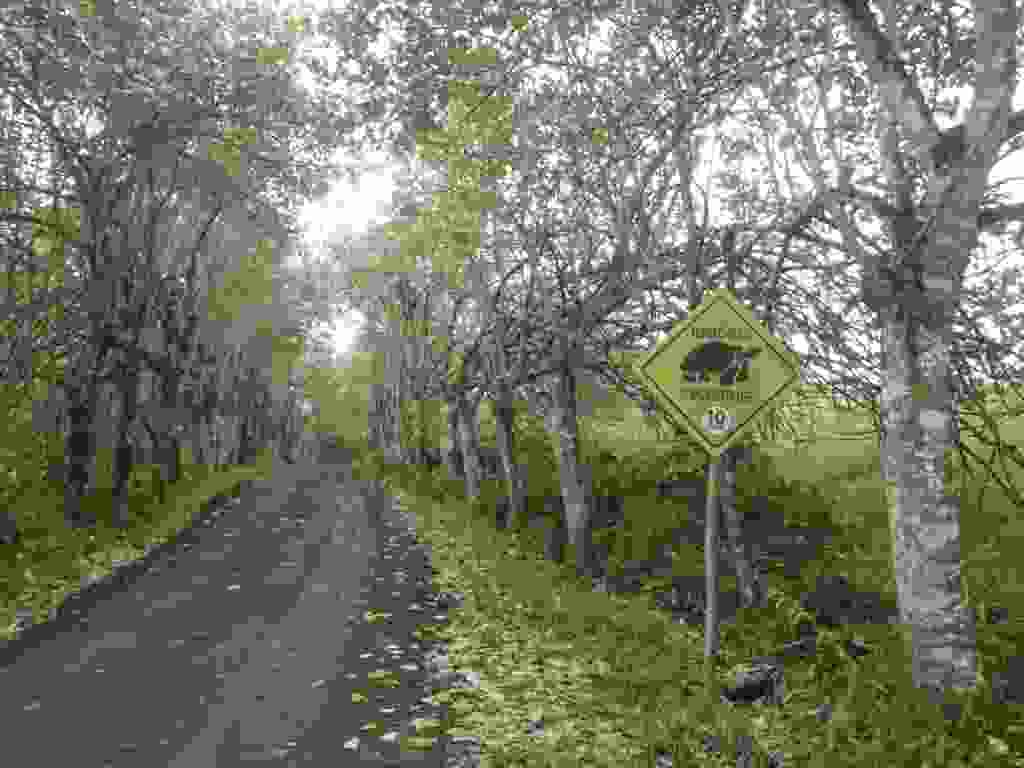
\includegraphics[width=\mywidth]{../wp-content/uploads/2015/07/P7025208-1024x768.jpg} \end{center}
\begin{center} 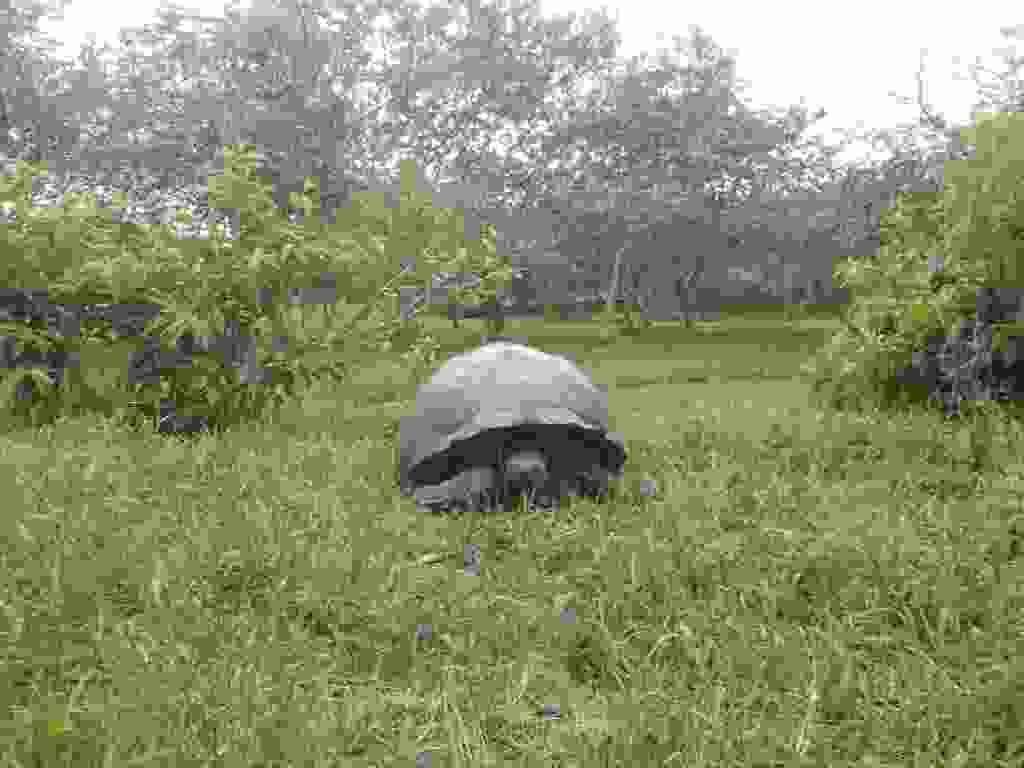
\includegraphics[width=\mywidth]{../wp-content/uploads/2015/07/P7025210-1024x768.jpg} \end{center}
\vfill
\begin{center} 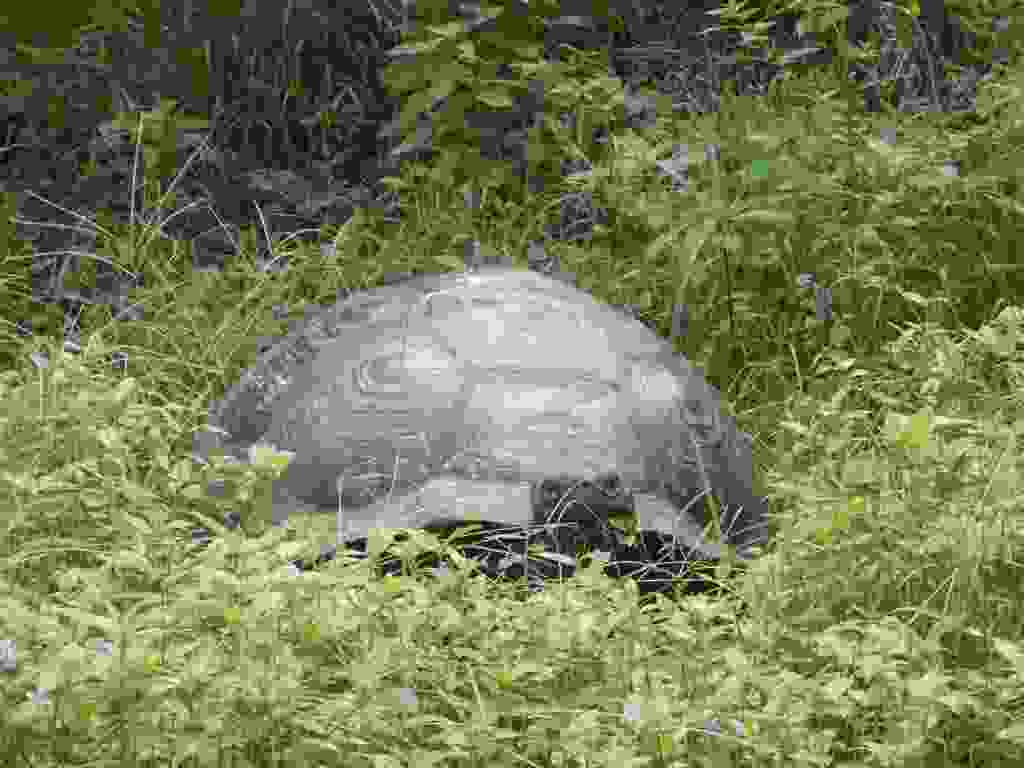
\includegraphics[width=\mywidth]{../wp-content/uploads/2015/07/P7025214-1024x768.jpg} \end{center}
\vspace{-\topsep}
\vspace{-0.75mm}
\pagebreak
~
\begin{center} 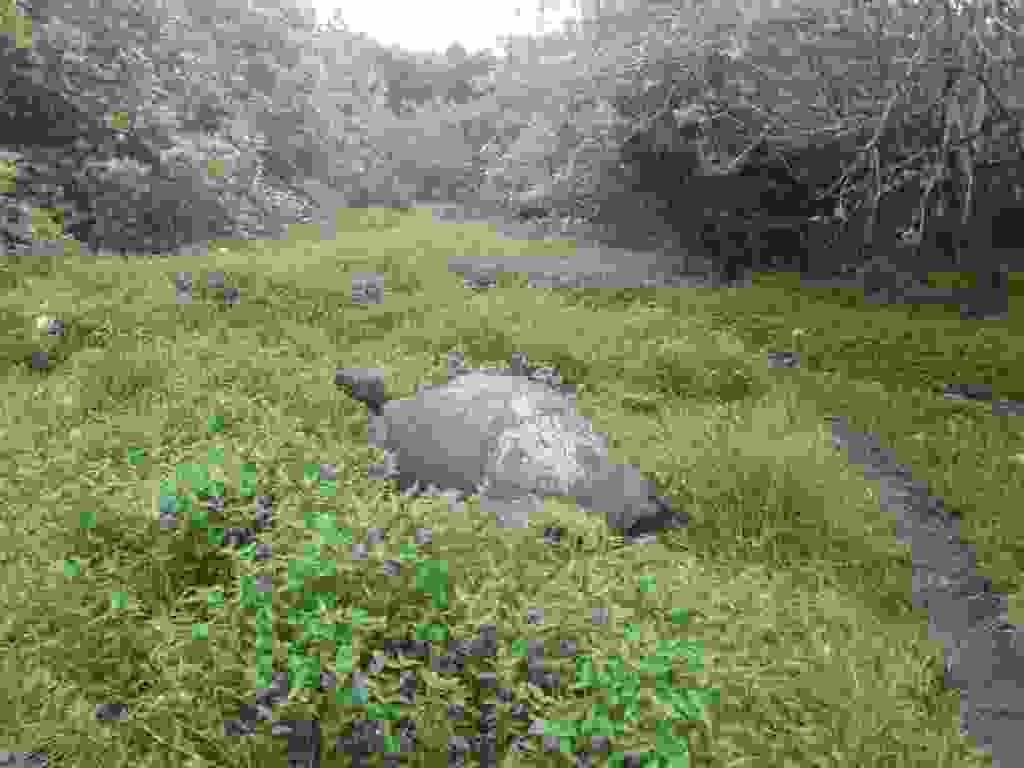
\includegraphics[width=\mywidth]{../wp-content/uploads/2015/07/P7025217-1024x768.jpg} \end{center}
~
\begin{center} 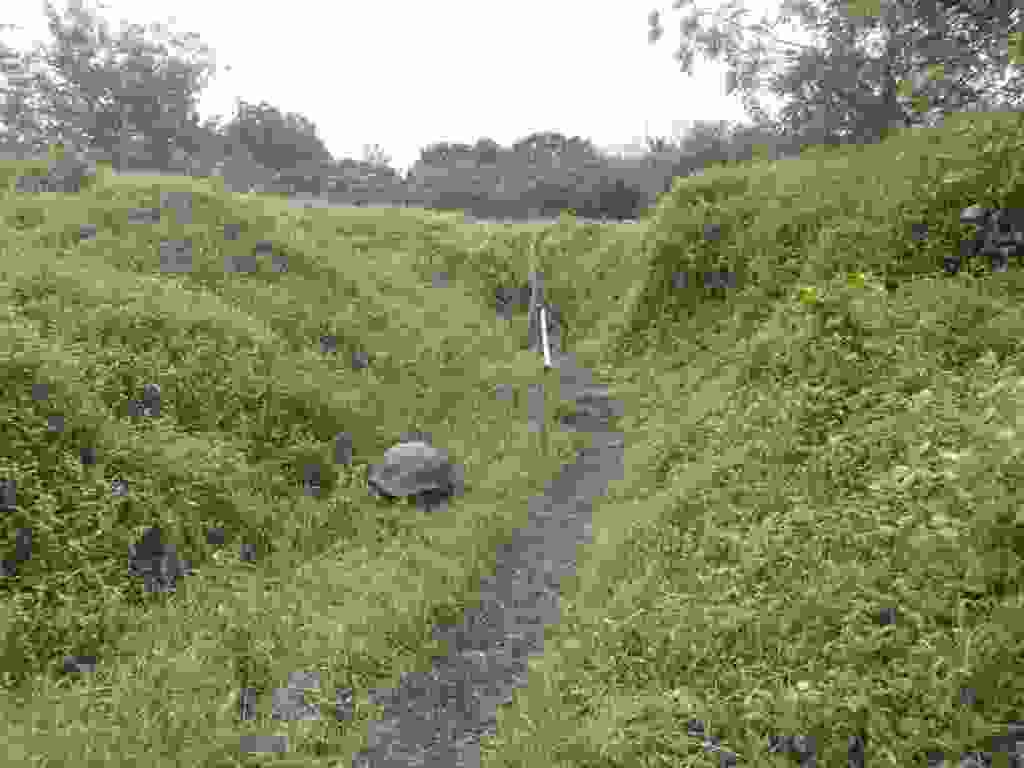
\includegraphics[width=\mywidth]{../wp-content/uploads/2015/07/P7025219-1024x768.jpg} \end{center}
\vspace{-\topsep}
\pagebreak

Il y aussi des tunnels de lave. 
\begin{center} 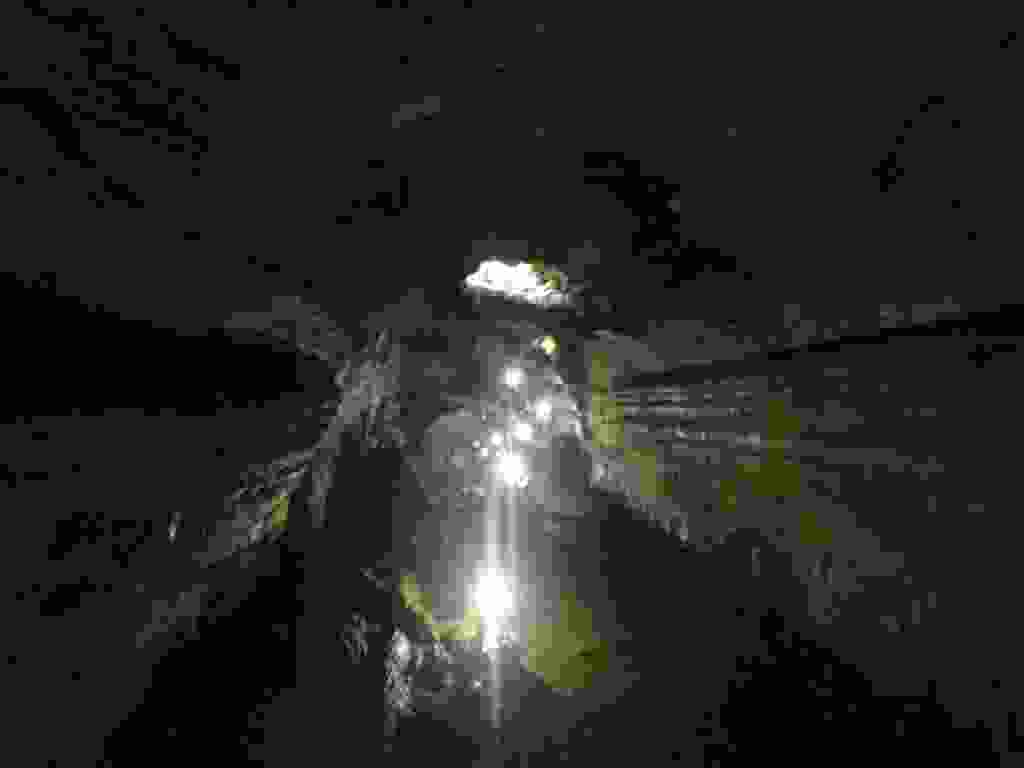
\includegraphics[width=\mywidth]{../wp-content/uploads/2015/07/P7025222-1024x768.jpg} \end{center}

Jolie balade jusqu'au site de Las Grietas. 
\begin{center} 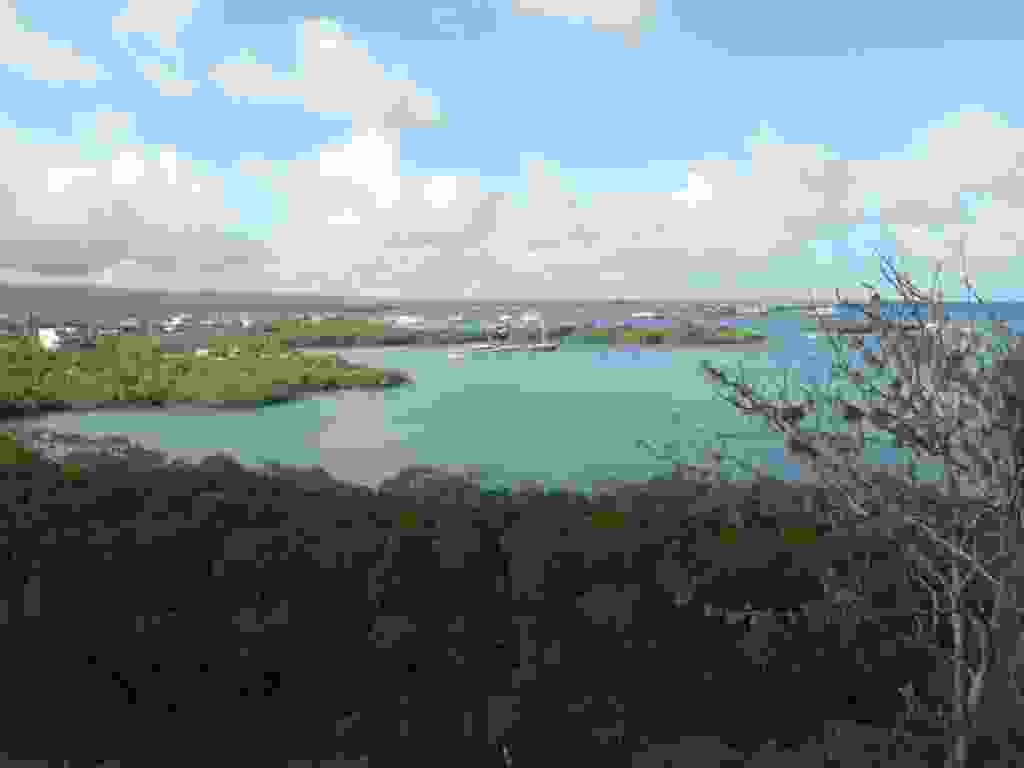
\includegraphics[width=\mywidth]{../wp-content/uploads/2015/07/P7035241-1024x768.jpg} \end{center}
\vspace{-\topsep}
\pagebreak

Petite plage, l'eau est bien chaude. 
\begin{center} 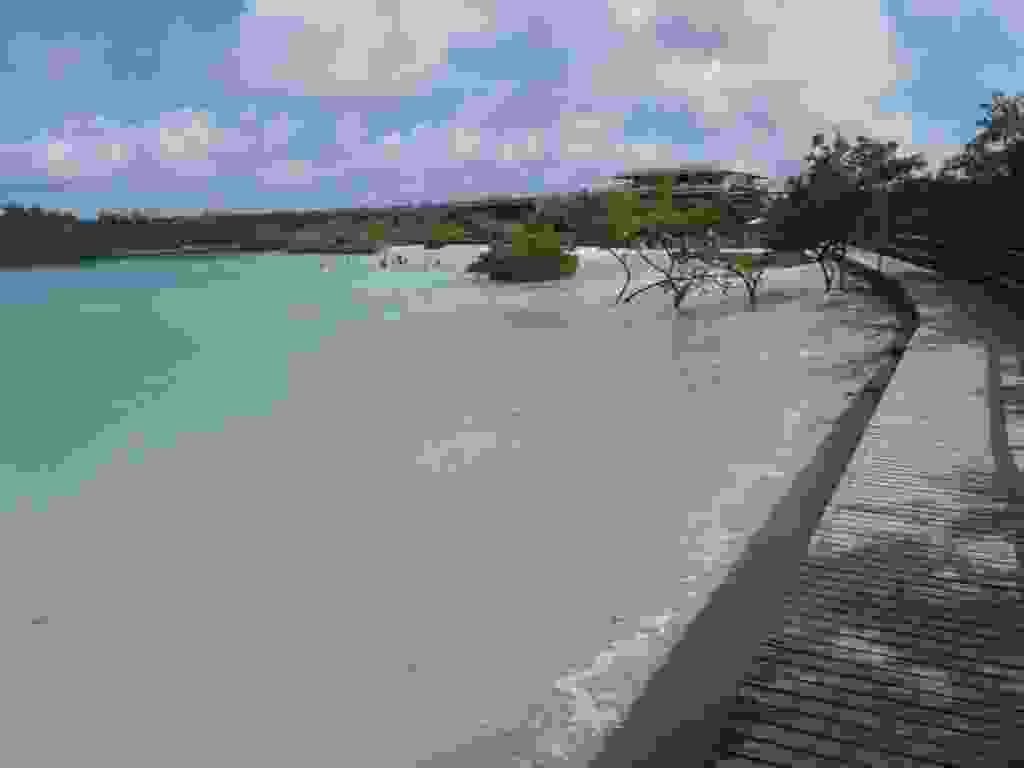
\includegraphics[width=\mywidth]{../wp-content/uploads/2015/07/P7025227-1024x768.jpg} \end{center}

Snorkeling dans la faille, pas beaucoup de poissons mais l'endroit est agréable. 
\begin{center} 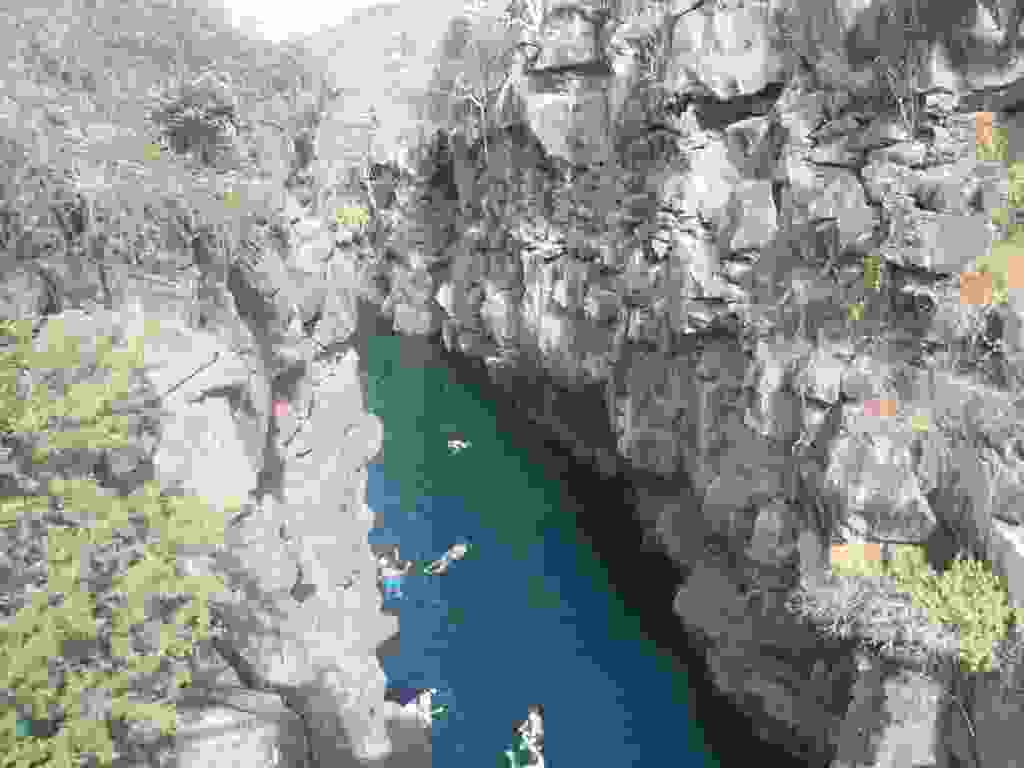
\includegraphics[width=\mywidth]{../wp-content/uploads/2015/07/P7025230-1024x768.jpg} \end{center}
\vspace{-\topsep}
\pagebreak
~
\begin{center} 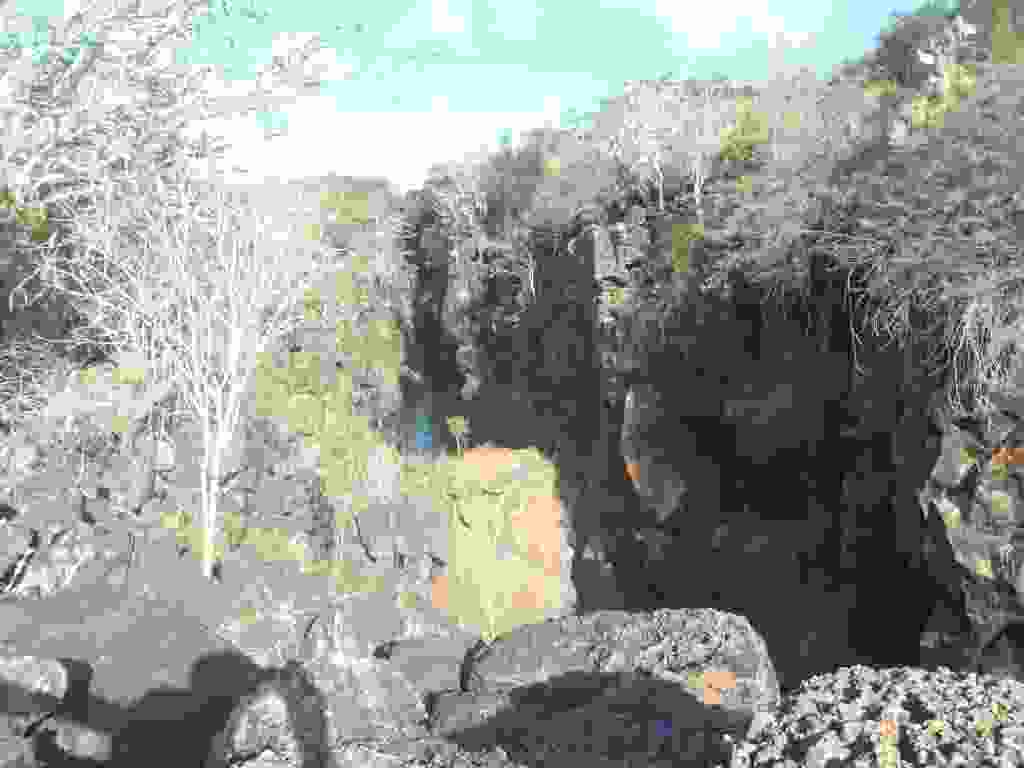
\includegraphics[width=\mywidth]{../wp-content/uploads/2015/07/P7035233-1024x768.jpg} \end{center}

Le lendemain je passe la journée à Tortuga Bay à 1h de marche de Puerto Ayora. 
\begin{center} 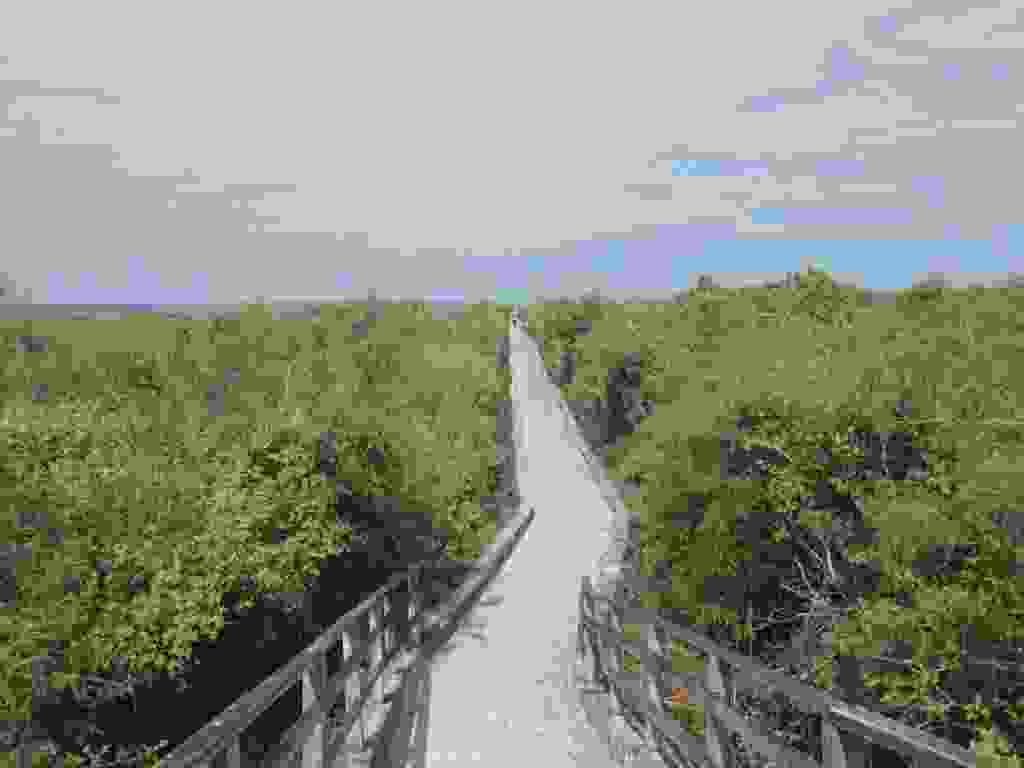
\includegraphics[width=\mywidth]{../wp-content/uploads/2015/07/P7035248-1024x768.jpg} \end{center}
\vspace{-\topsep}
\pagebreak
~\\
\begin{center} 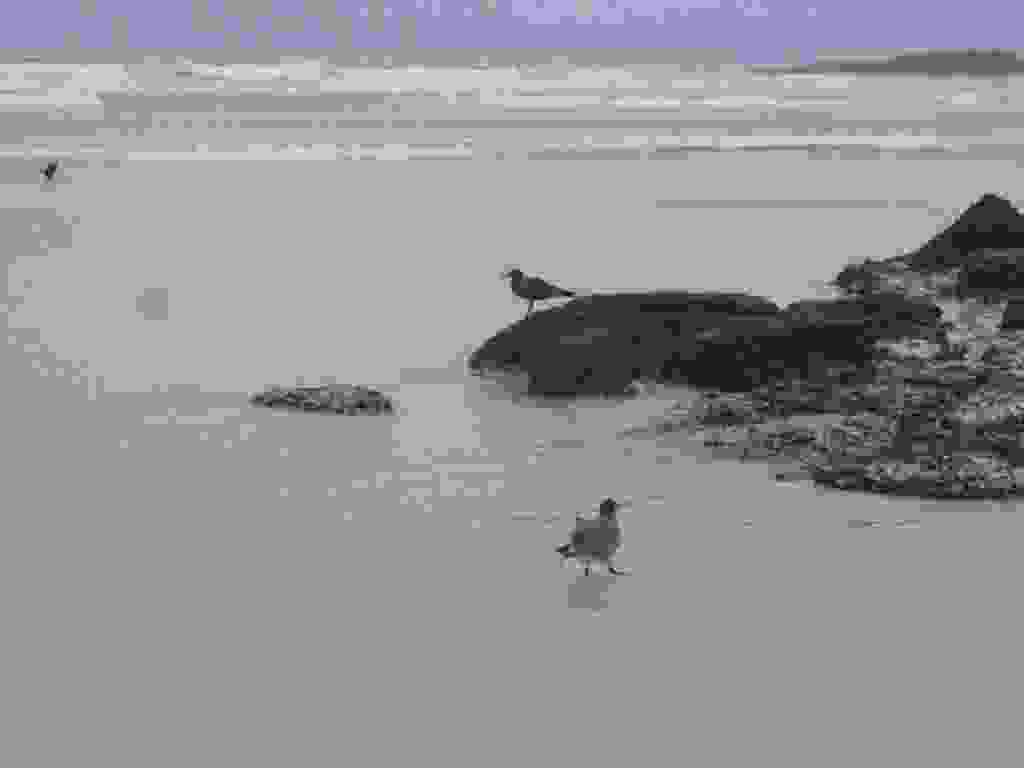
\includegraphics[width=\mywidth]{../wp-content/uploads/2015/07/P7035253-1024x768.jpg} \end{center}
\begin{center} 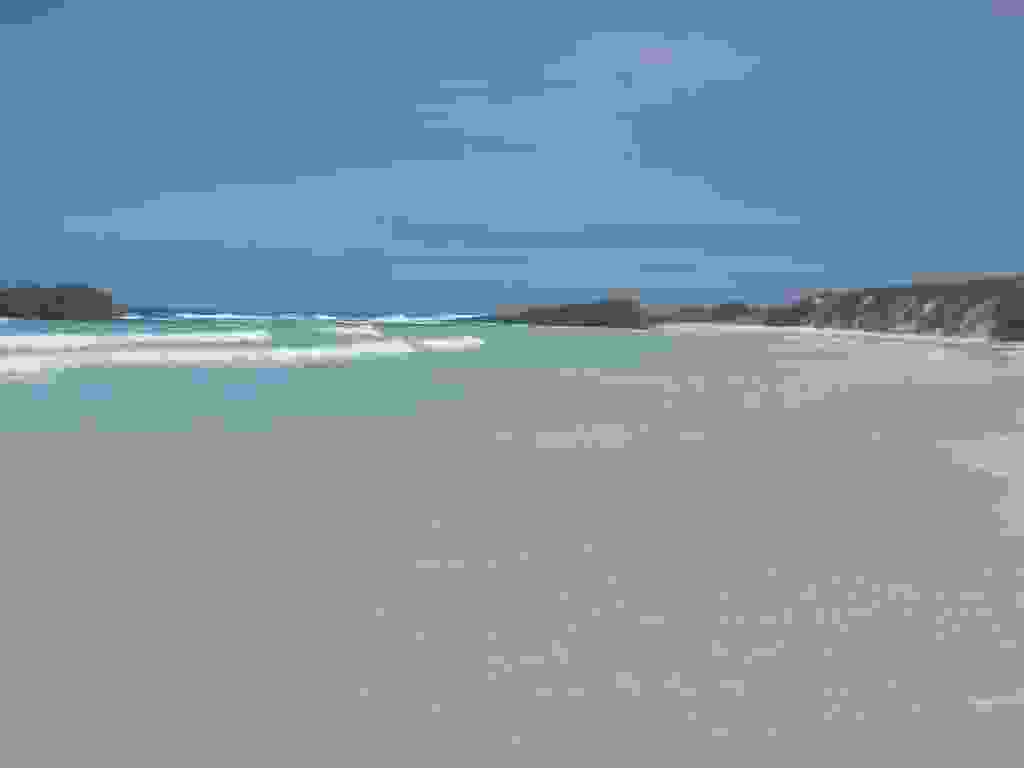
\includegraphics[width=\mywidth]{../wp-content/uploads/2015/07/P7035280-1024x768.jpg} \end{center}
\vspace{-\topsep}
\vspace{-2.75mm}
\pagebreak

Beaucoup d'iguanes mais pas de tortues, en fait elle viennent sur la plage seulement pour déposer leurs oeufs. 
\begin{center} 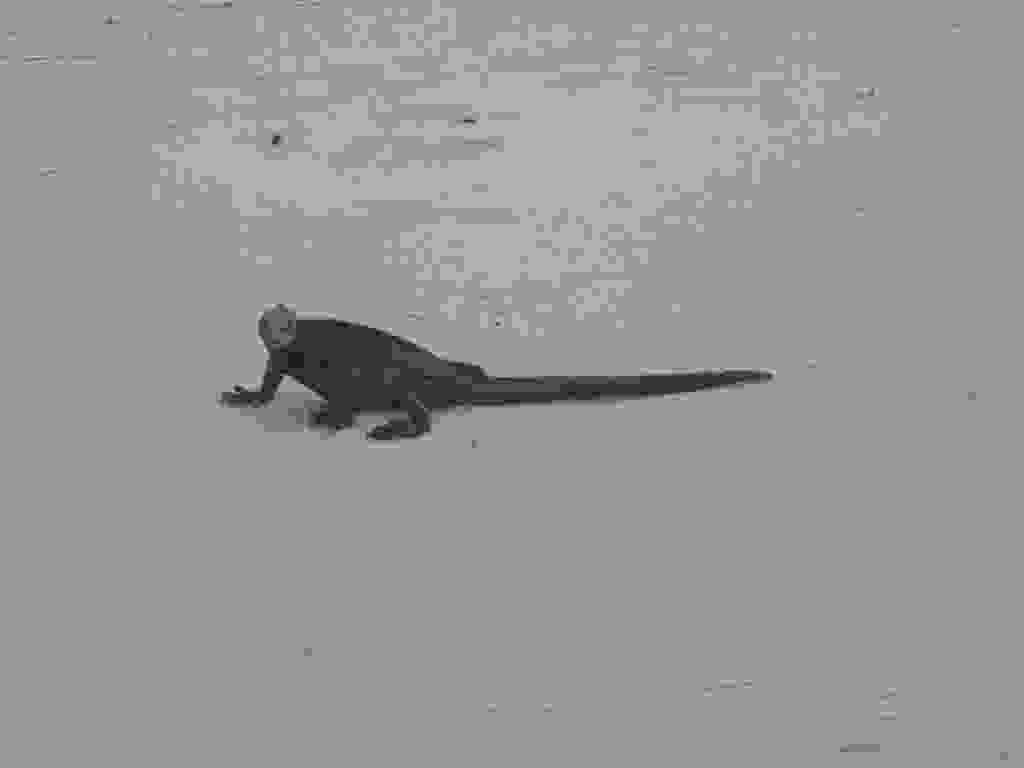
\includegraphics[width=\mywidth]{../wp-content/uploads/2015/07/P7035255-1024x768.jpg} \end{center}
\begin{center} 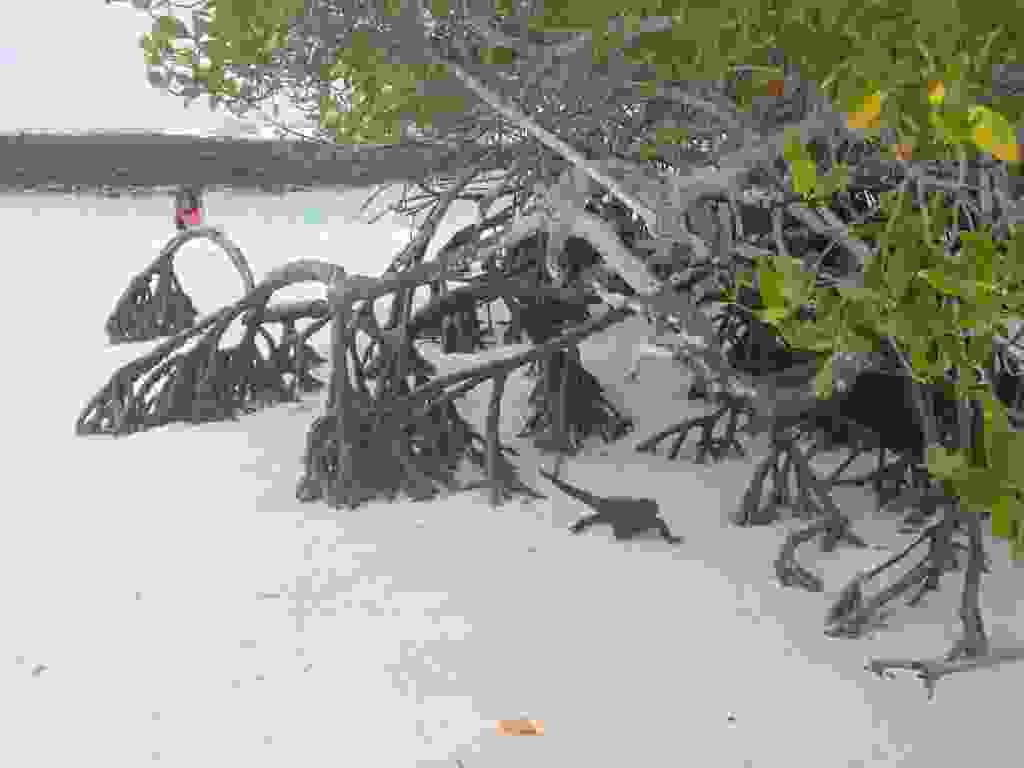
\includegraphics[width=\mywidth]{../wp-content/uploads/2015/07/P7035260-1024x768.jpg} \end{center}
\vspace{-\topsep}
\vspace{-2.75mm}
\pagebreak
~\\
\begin{center} 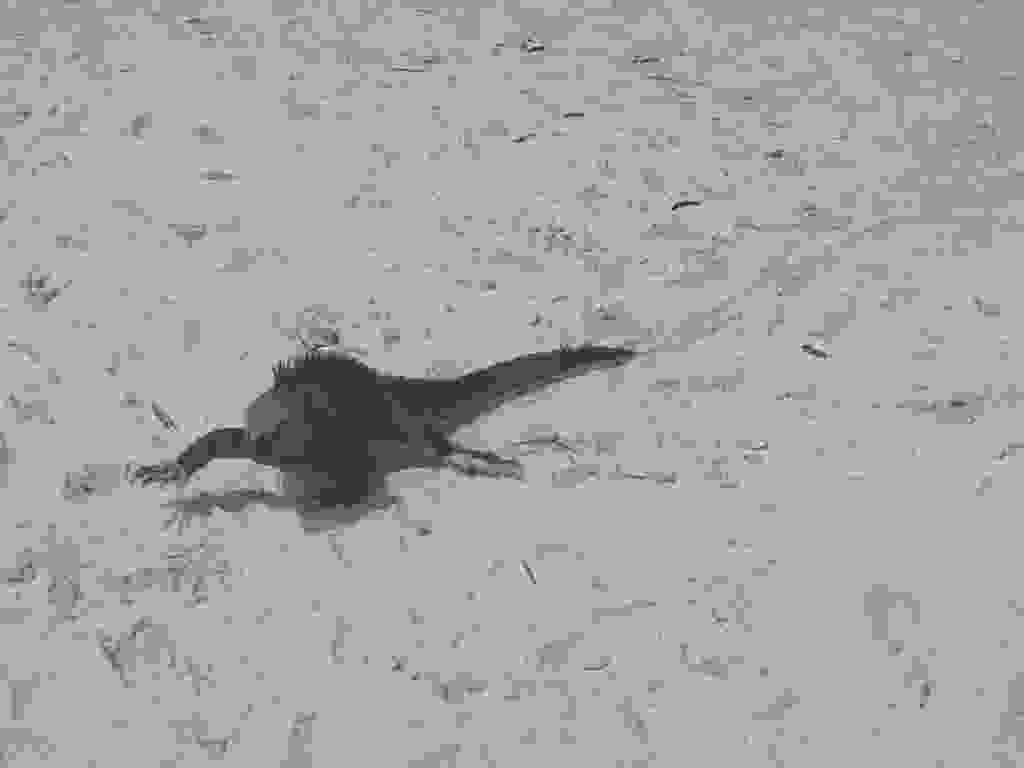
\includegraphics[width=\mywidth]{../wp-content/uploads/2015/07/P7035275-1024x768.jpg} \end{center}

Je tente le snorkeling mais l'eau est bien trouble. 
\begin{center} 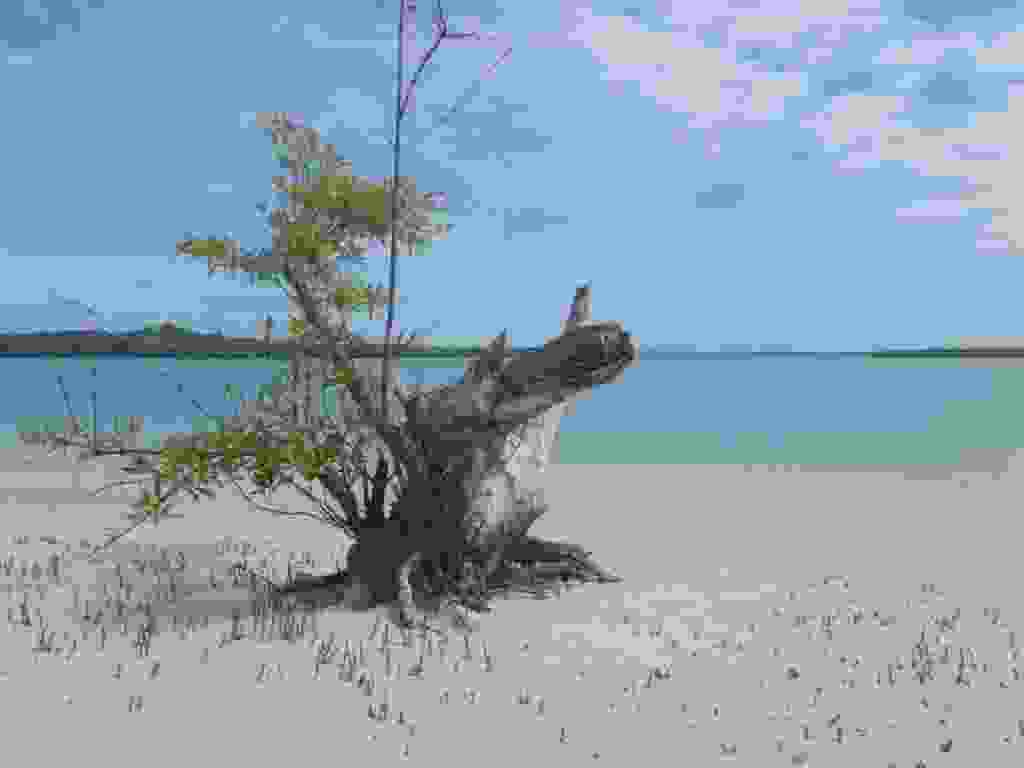
\includegraphics[width=\mywidth]{../wp-content/uploads/2015/07/P7035272-1024x768.jpg} \end{center}
\vspace{-\topsep}
\pagebreak

Après 3 jours sur l'île de Santa Cruz, je passe sur l'île d'Isabela qui est la plus grande des Galapagos. 
\begin{center} 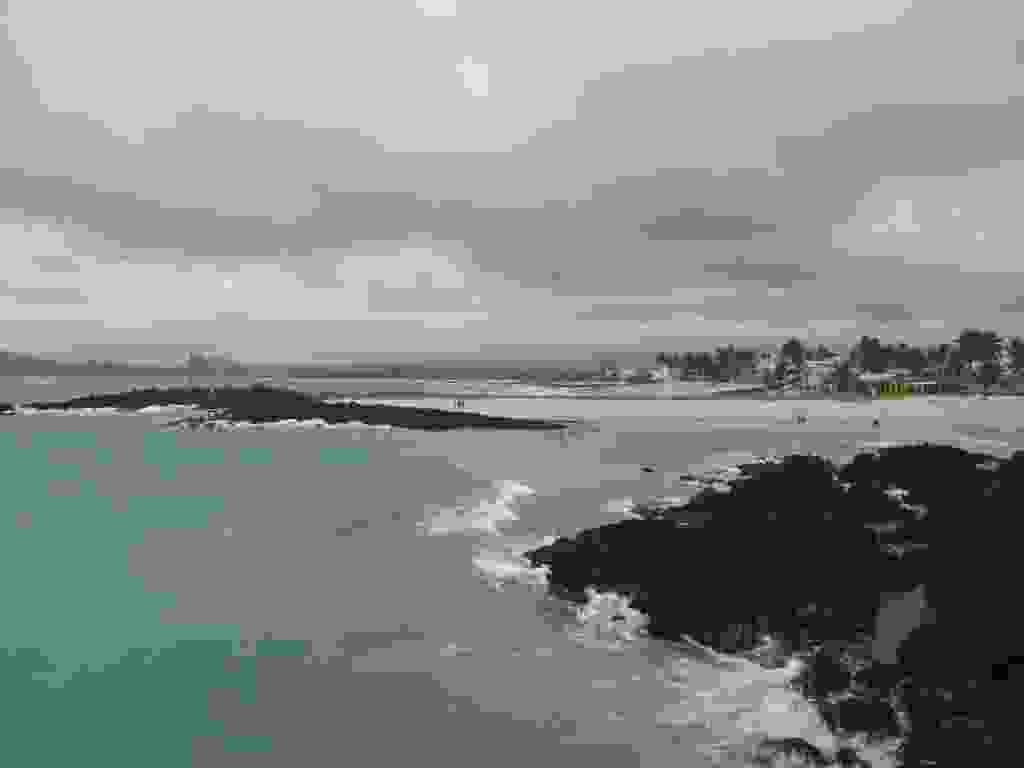
\includegraphics[width=\mywidth]{../wp-content/uploads/2015/07/P7045281-1024x768.jpg} \end{center}
~
\begin{center} 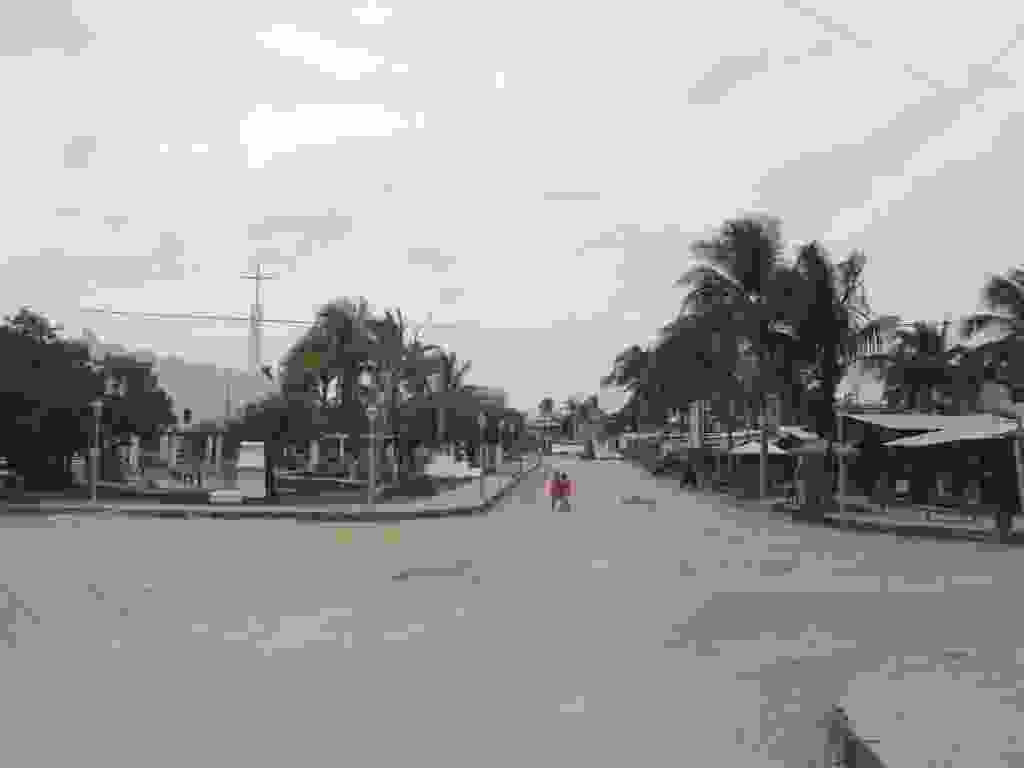
\includegraphics[width=\mywidth]{../wp-content/uploads/2015/07/P7045285-1024x768.jpg} \end{center}
\vspace{-\topsep}
\pagebreak

5km à pied pour voir le mur des larmes construit par des prisonniers à l'époque où l'île servait de bagne. 
\begin{center} 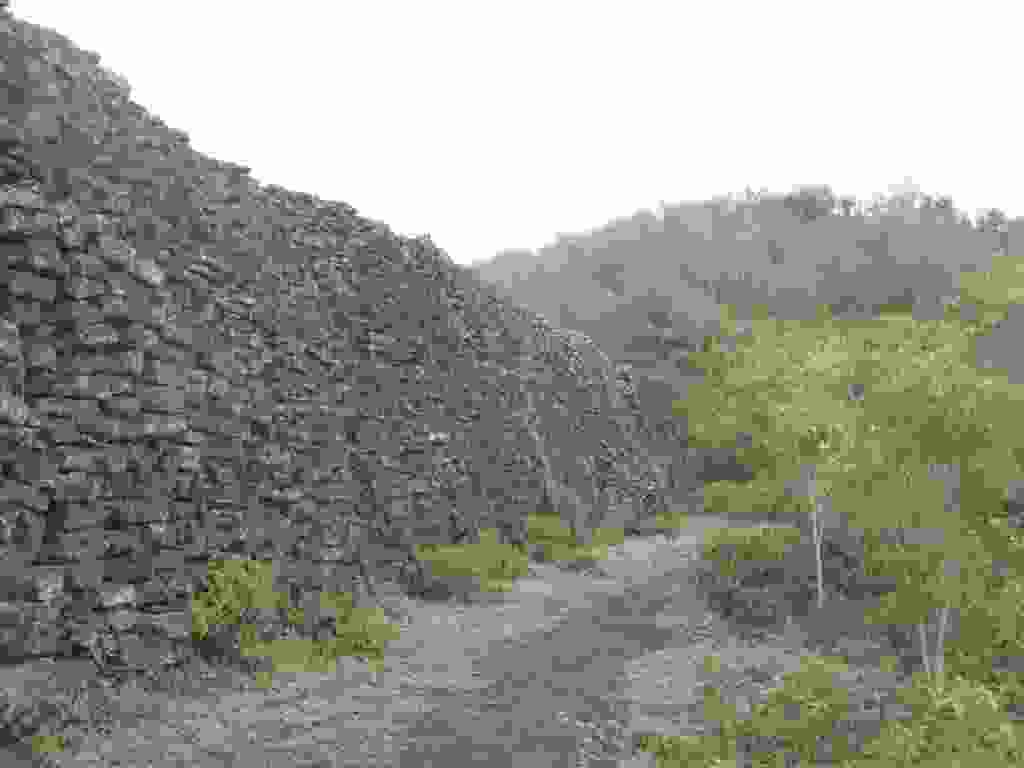
\includegraphics[width=\mywidth]{../wp-content/uploads/2015/07/P7045317-1024x768.jpg} \end{center}

En chemin, des belles plages et des dizaines d'iguanes. 
\begin{center} 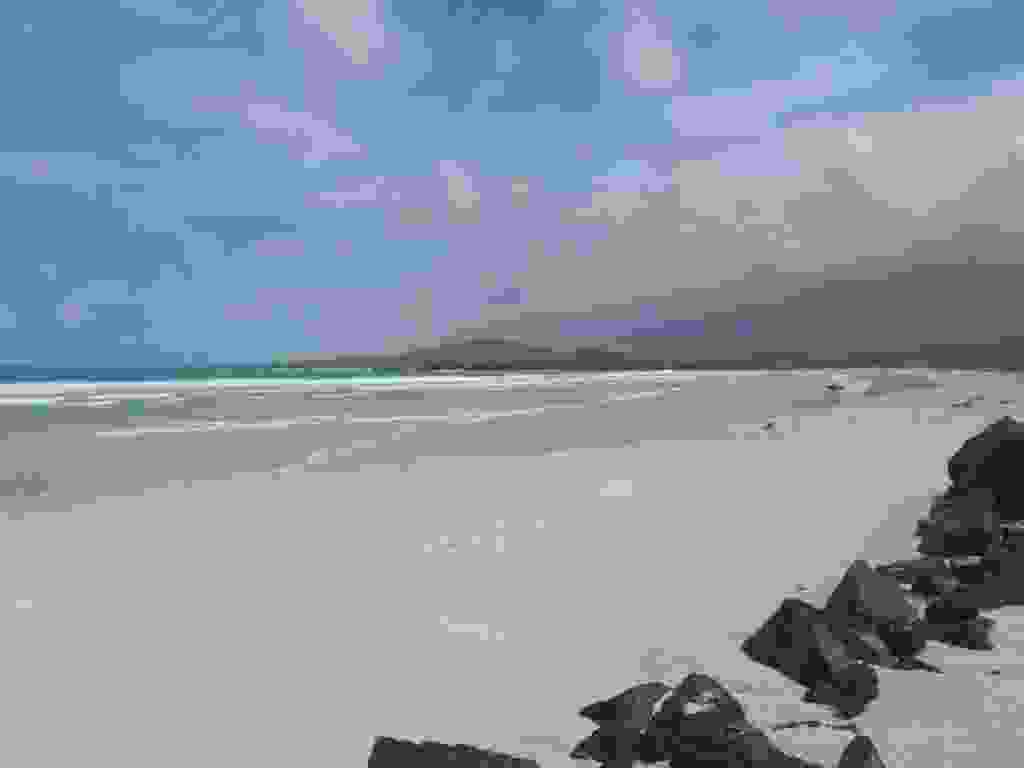
\includegraphics[width=\mywidth]{../wp-content/uploads/2015/07/P7045289-1024x768.jpg} \end{center}
\vspace{-\topsep}
\pagebreak
~\\
\begin{center} 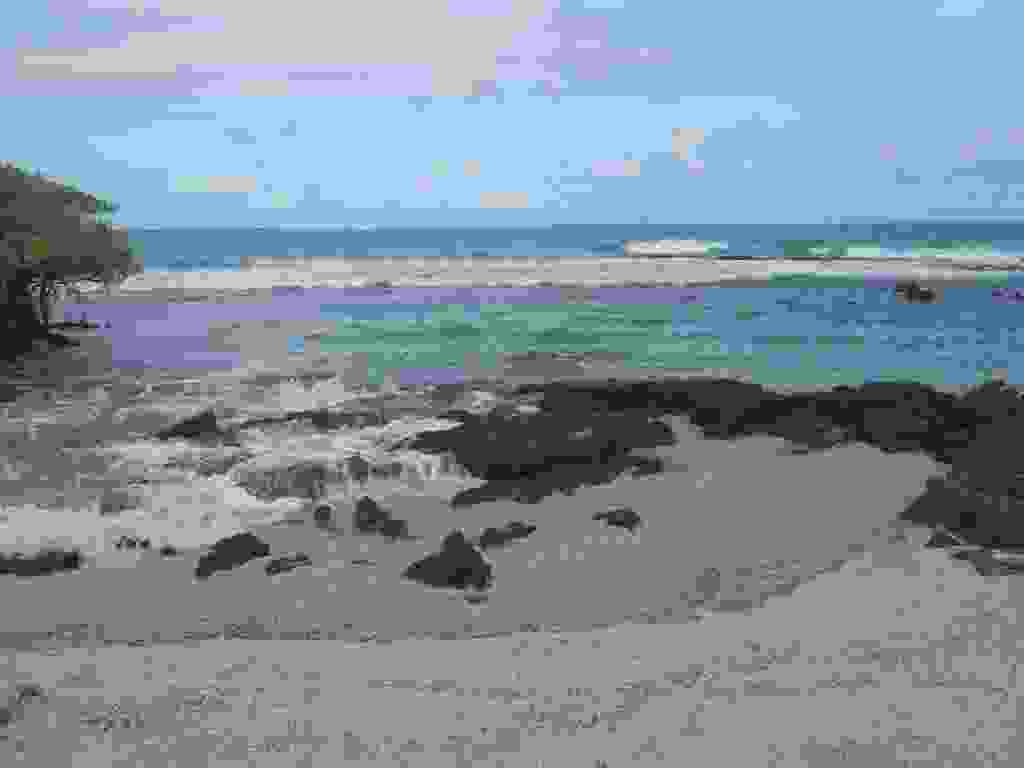
\includegraphics[width=\mywidth]{../wp-content/uploads/2015/07/P7045324-1024x768.jpg} \end{center}
~
\begin{center} 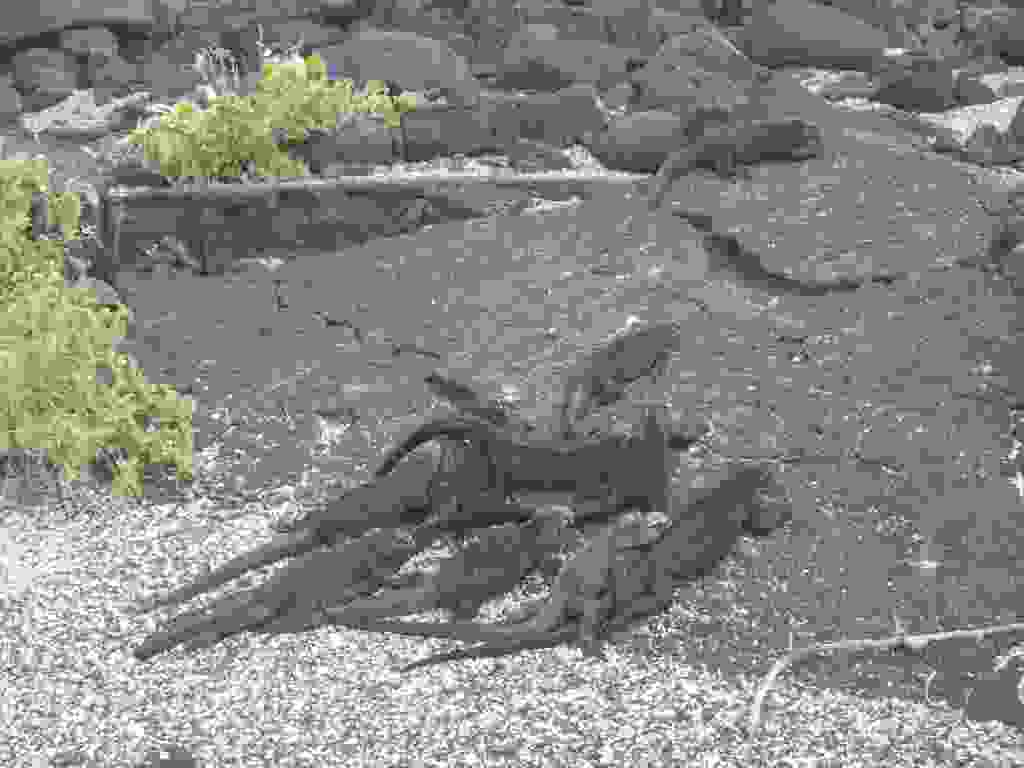
\includegraphics[width=\mywidth]{../wp-content/uploads/2015/07/P7045326-1024x768.jpg} \end{center}
\vspace{-\topsep}
\pagebreak
~
\begin{center} 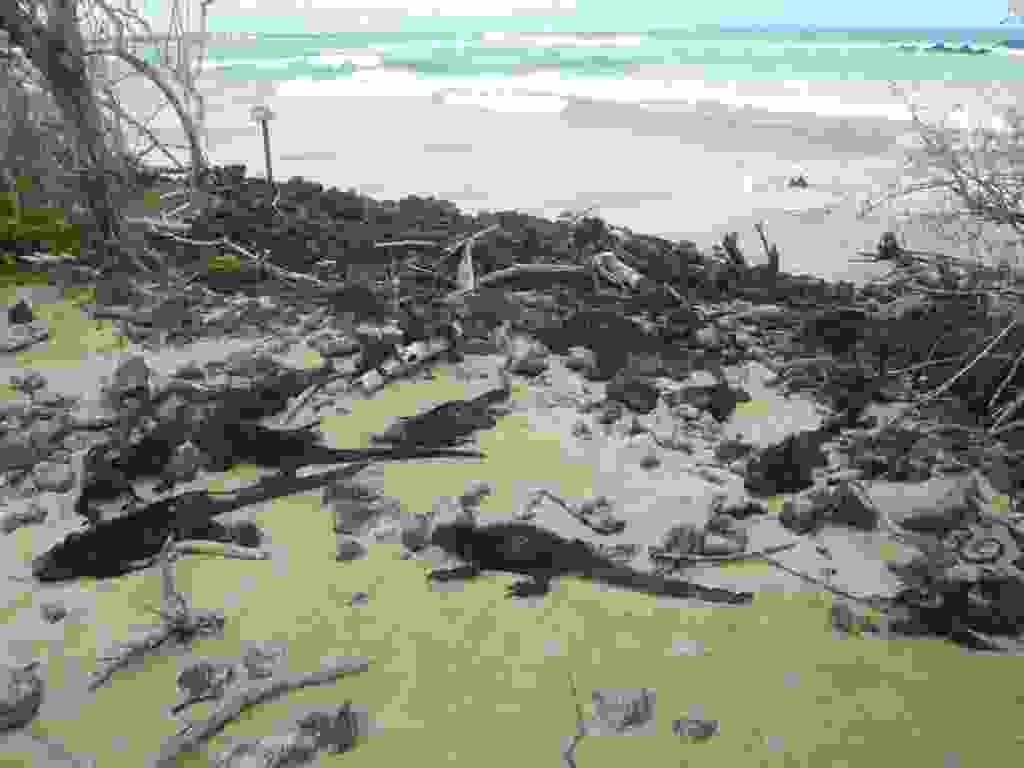
\includegraphics[width=\mywidth]{../wp-content/uploads/2015/07/P7045330-1024x768.jpg} \end{center}
\begin{center} 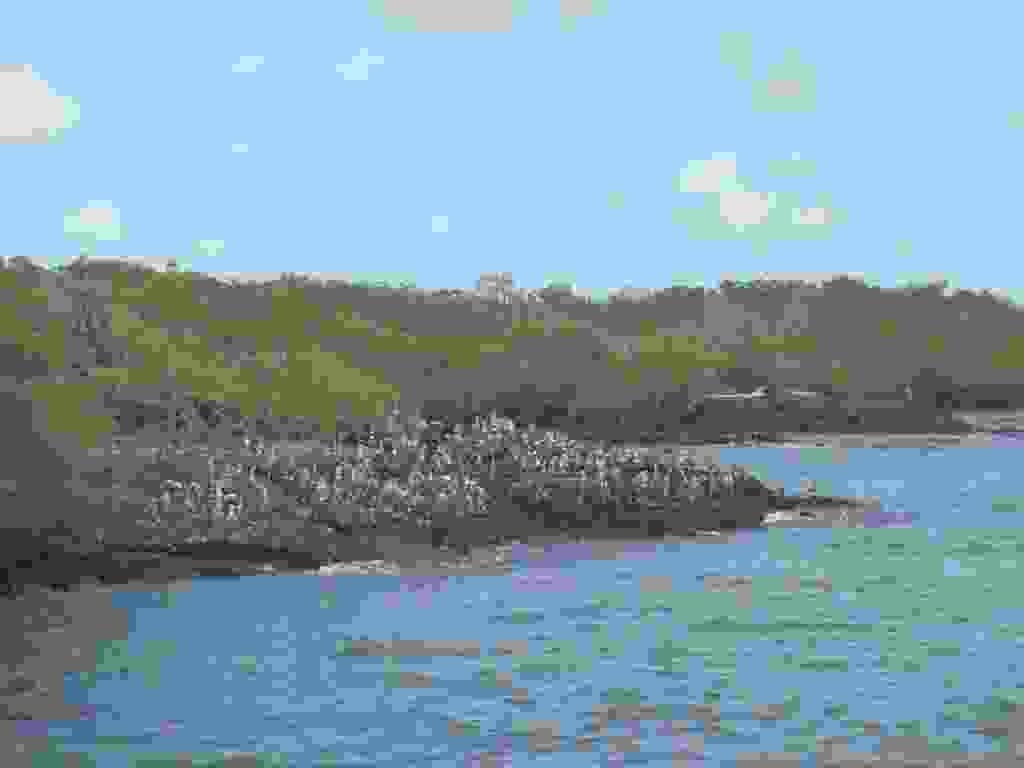
\includegraphics[width=\mywidth]{../wp-content/uploads/2015/07/P7045299-1024x768.jpg} \end{center}
\vspace{-\topsep}
\vspace{-3.25mm}
\pagebreak

Quelques tortues. 
\begin{center} 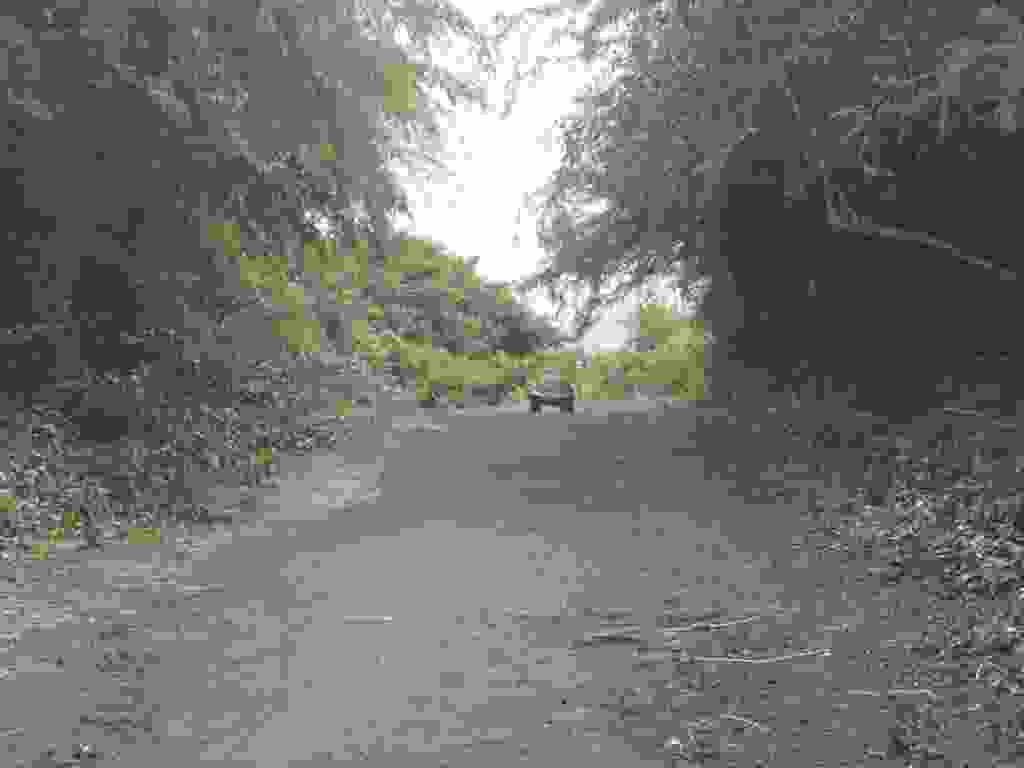
\includegraphics[width=\mywidth]{../wp-content/uploads/2015/07/P7045305-1024x768.jpg} \end{center}
\begin{center} 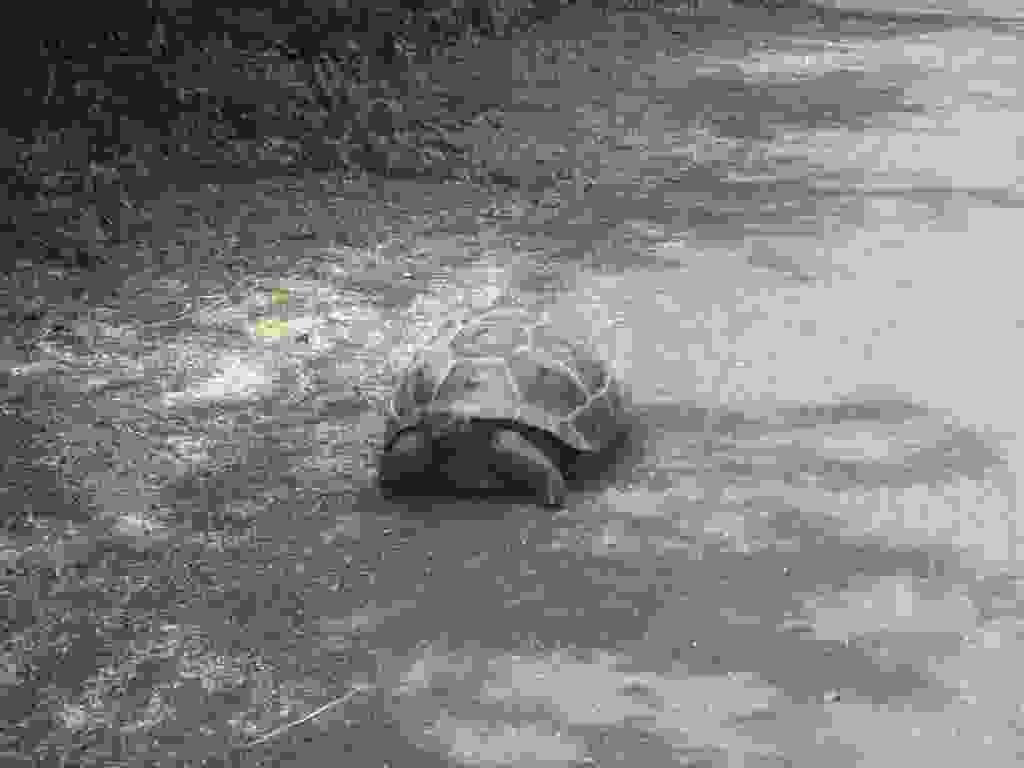
\includegraphics[width=\mywidth]{../wp-content/uploads/2015/07/P7045309-1024x768.jpg} \end{center}
\begin{center} 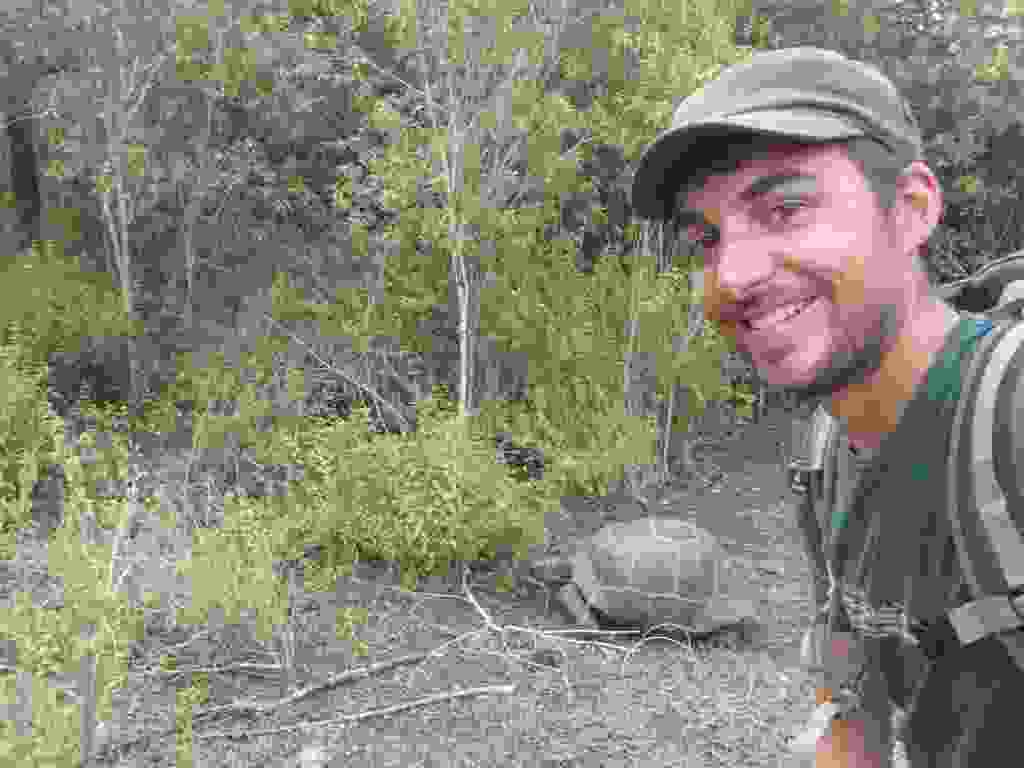
\includegraphics[width=\mywidth]{../wp-content/uploads/2015/07/P7045321-1024x768.jpg} \end{center}

Le chemin traverse une zone humide de l'île, avec la mangrove. 
\begin{center} 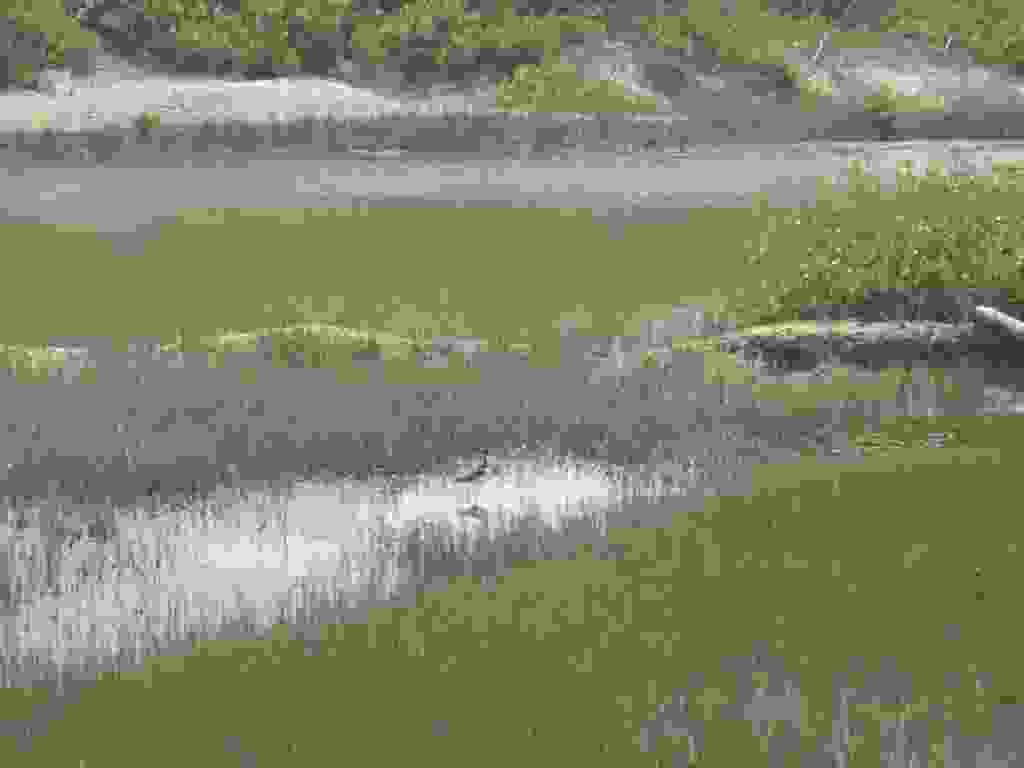
\includegraphics[width=\mywidth]{../wp-content/uploads/2015/07/P7045290-1024x768.jpg} \end{center}
\begin{center} 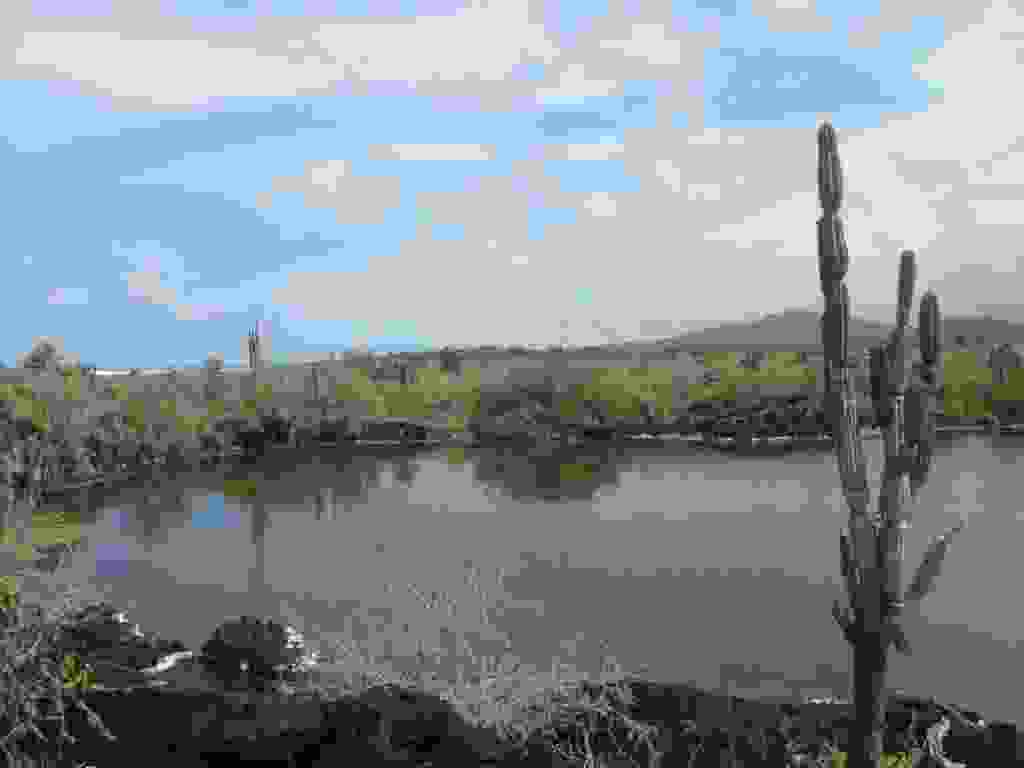
\includegraphics[width=\mywidth]{../wp-content/uploads/2015/07/P7045293-1024x768.jpg} \end{center}
\vfill
\begin{center} 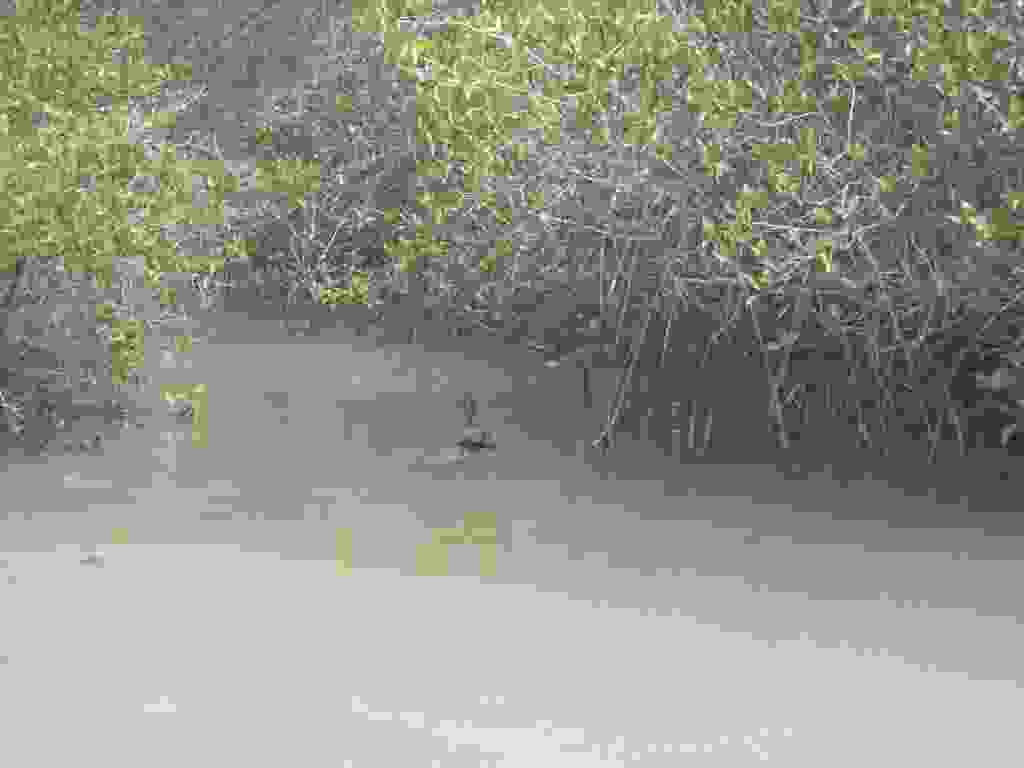
\includegraphics[width=\mywidth]{../wp-content/uploads/2015/07/P7045304-1024x768.jpg} \end{center}
\vspace{-\topsep}
\vspace{-0.75mm}
\pagebreak

Un tunnel de lave. 
\begin{center} 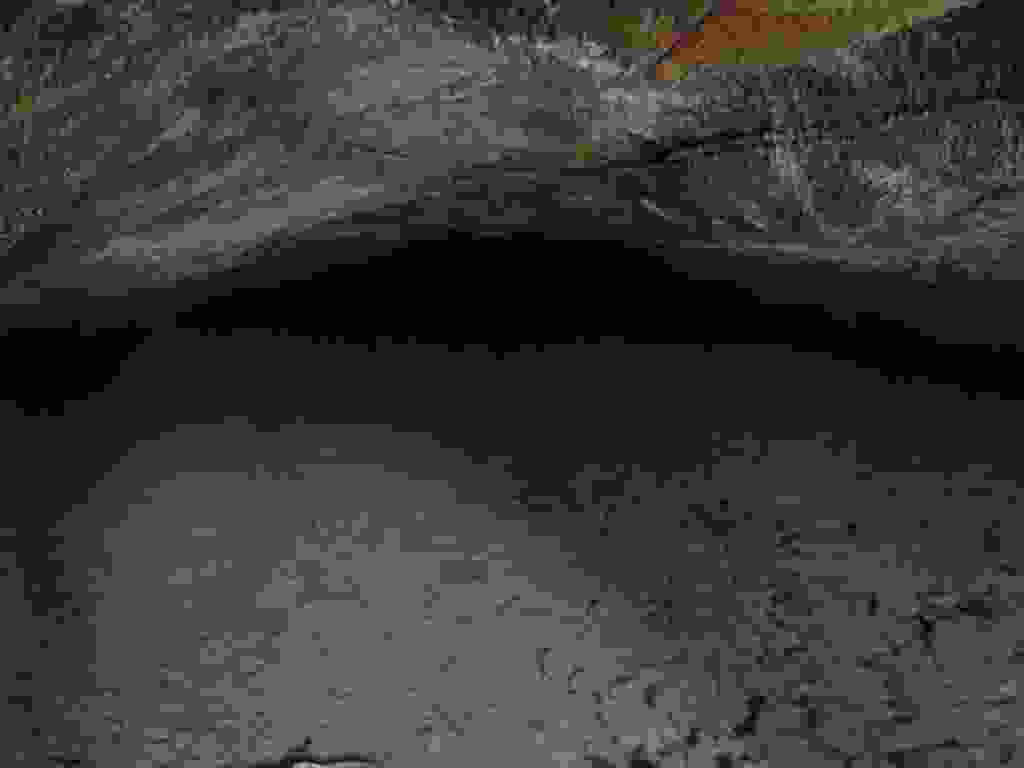
\includegraphics[width=\mywidth]{../wp-content/uploads/2015/07/P7045294-1024x768.jpg} \end{center}

Mirador avec beau point de vue. 
\begin{center} 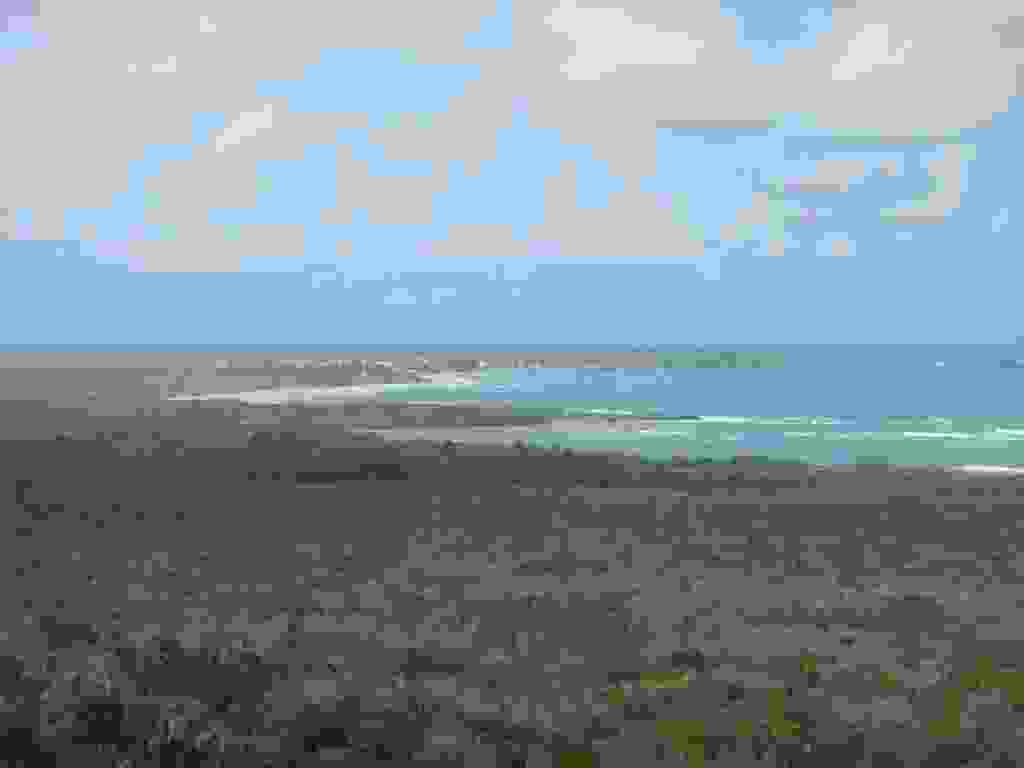
\includegraphics[width=\mywidth]{../wp-content/uploads/2015/07/P7045314-1024x768.jpg} \end{center}
\vspace{-\topsep}
\pagebreak
~
\begin{center} 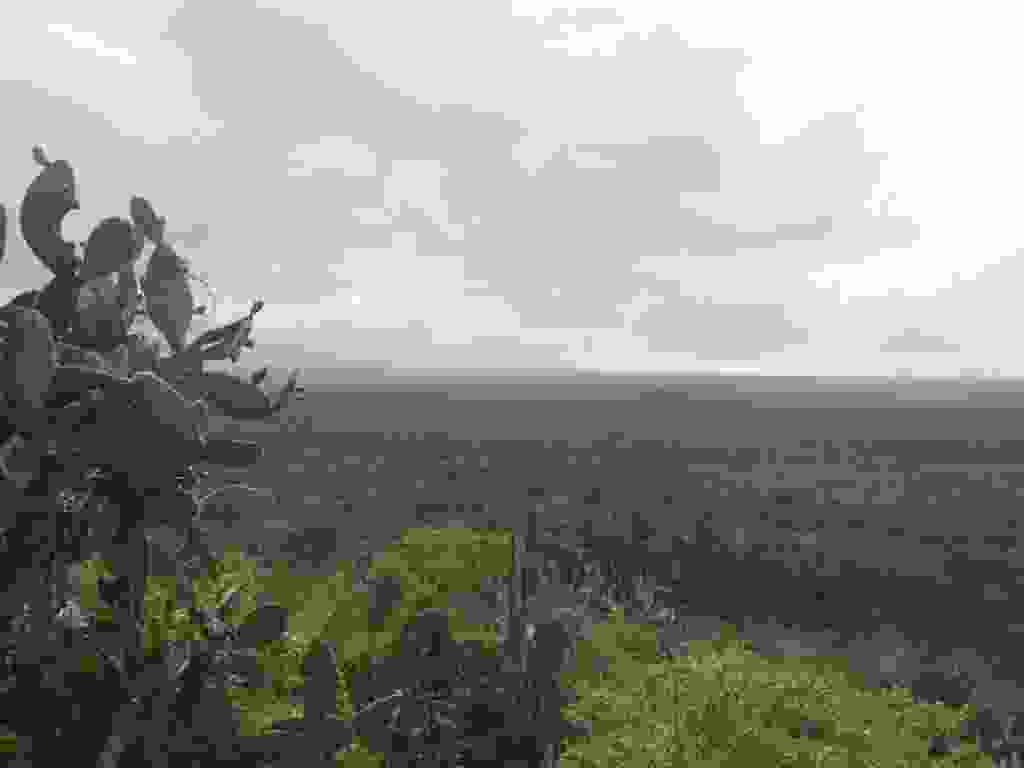
\includegraphics[width=\mywidth]{../wp-content/uploads/2015/07/P7045312-1024x768.jpg} \end{center}

Je finis la journée à Concha de Perla où je croise quelques phoques. 
\begin{center} 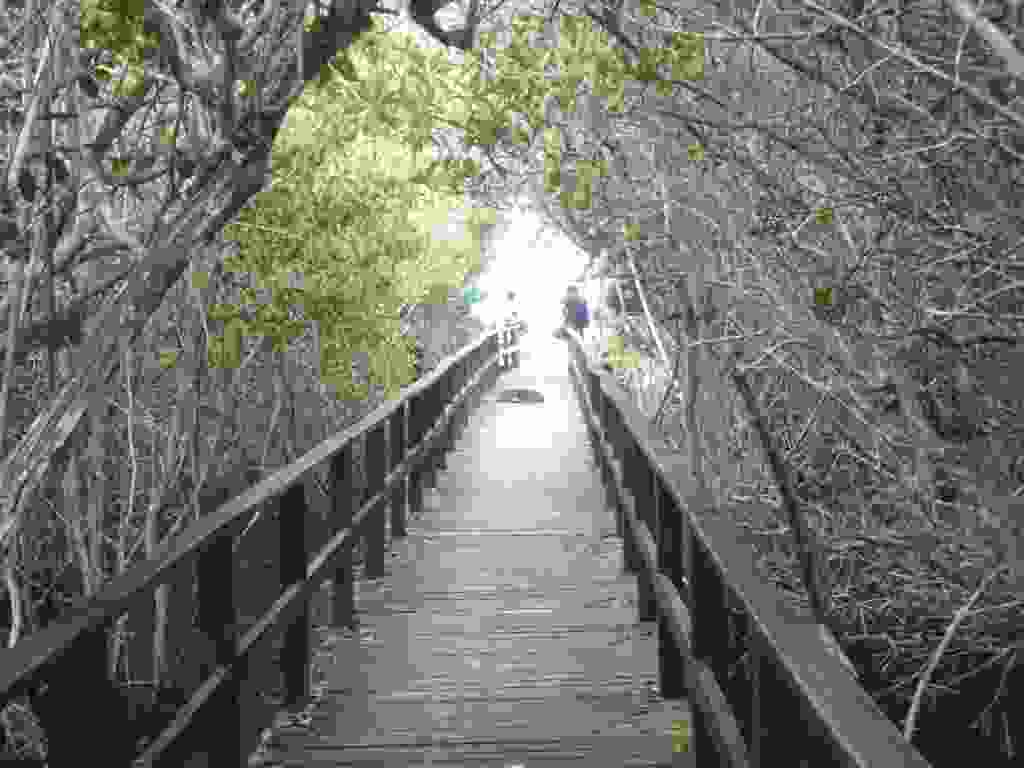
\includegraphics[width=\mywidth]{../wp-content/uploads/2015/07/P7055337-1024x768.jpg} \end{center}
\vspace{-\topsep}
\pagebreak
~\\
\begin{center} 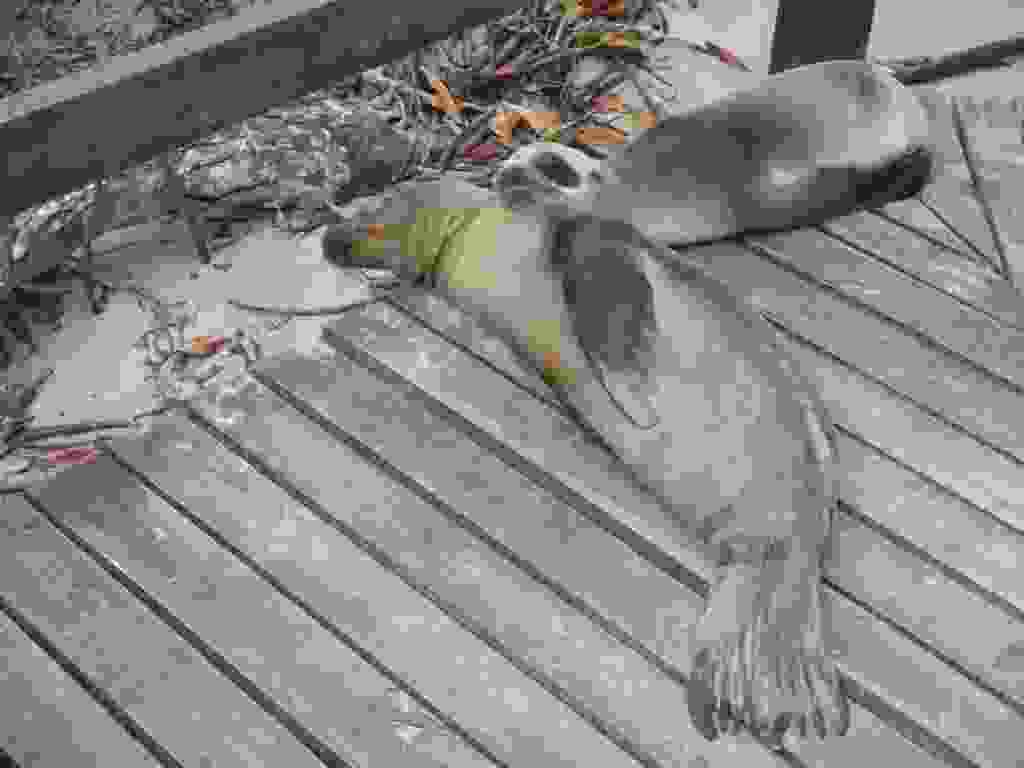
\includegraphics[width=\mywidth]{../wp-content/uploads/2015/07/P7055335-1024x768.jpg} \end{center}
\begin{center} 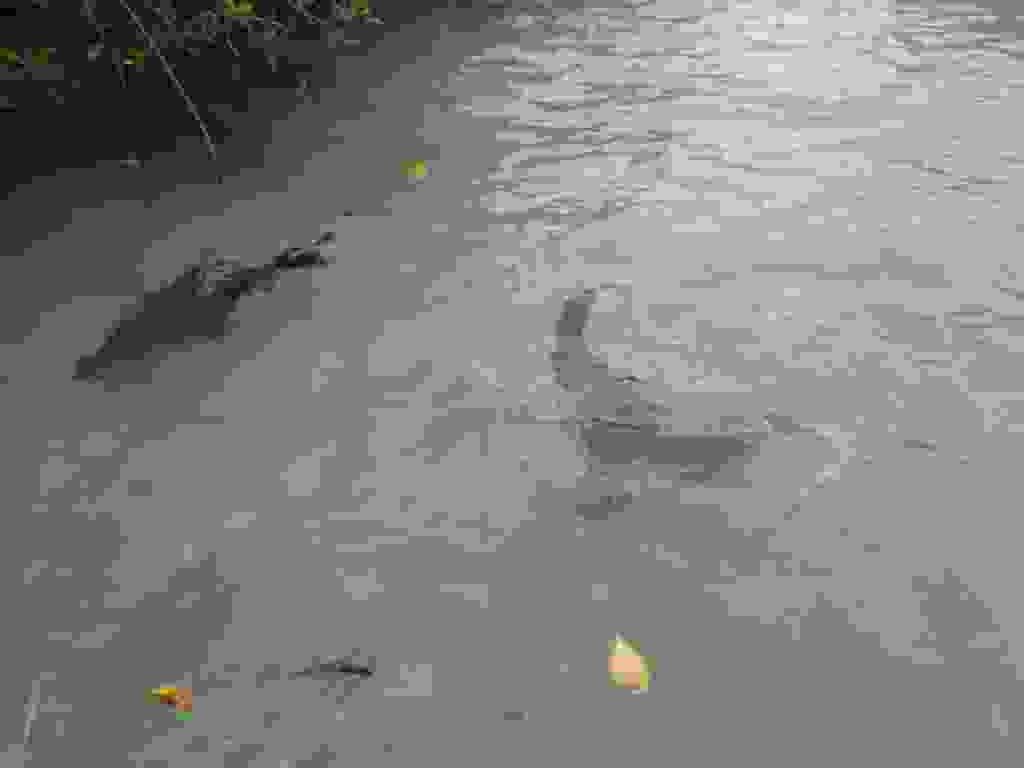
\includegraphics[width=\mywidth]{../wp-content/uploads/2015/07/P7055334-1024x768.jpg} \end{center}
\vspace{-\topsep}
\vspace{-2.75mm}
\pagebreak

Le lendemain montée au volcan Sierra Negra qui a le 2\ieme\ plus grand cratère du monde. 
\begin{center} 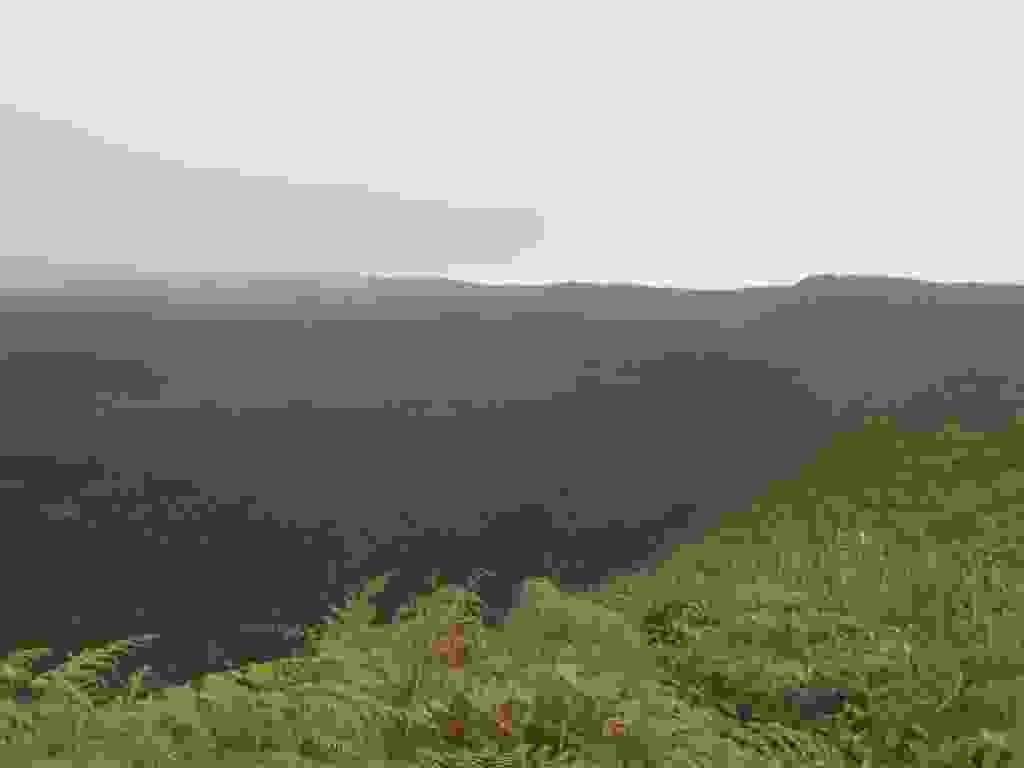
\includegraphics[width=\mywidth]{../wp-content/uploads/2015/07/P7055345-1024x768.jpg} \end{center}
\begin{center} 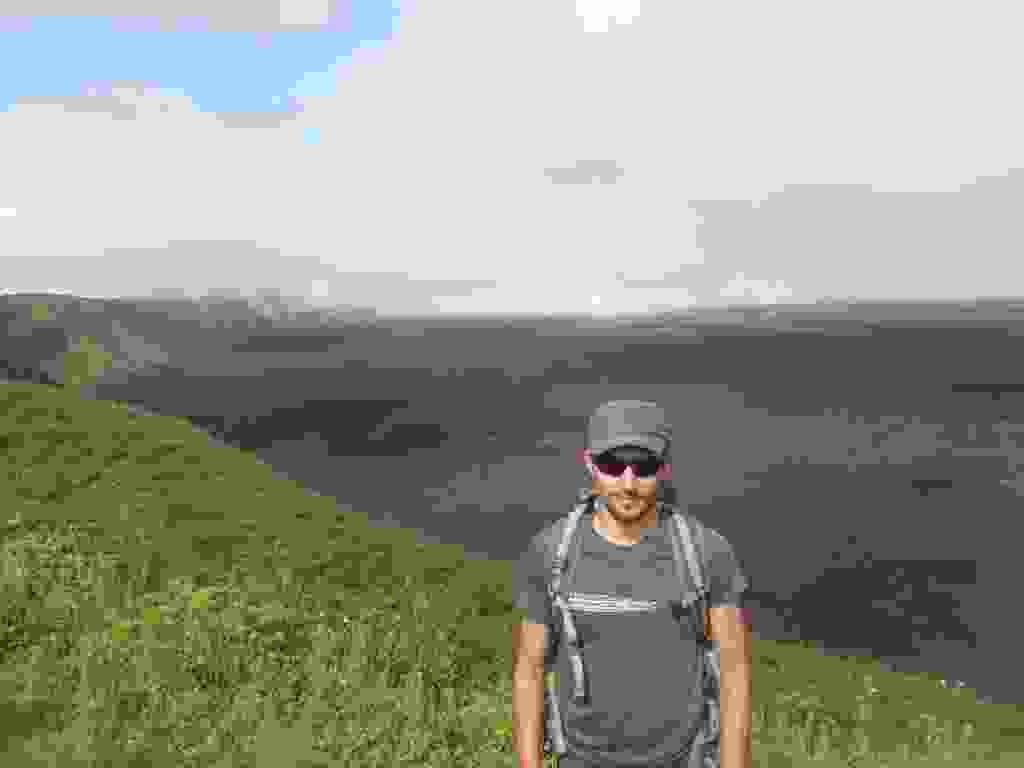
\includegraphics[width=\mywidth]{../wp-content/uploads/2015/07/P7055351-1024x768.jpg} \end{center}
\vspace{-\topsep}
\vspace{-2.75mm}
\pagebreak

Un peu plus loin le volcan El Chico avec des paysages lunaires. 
\begin{center} 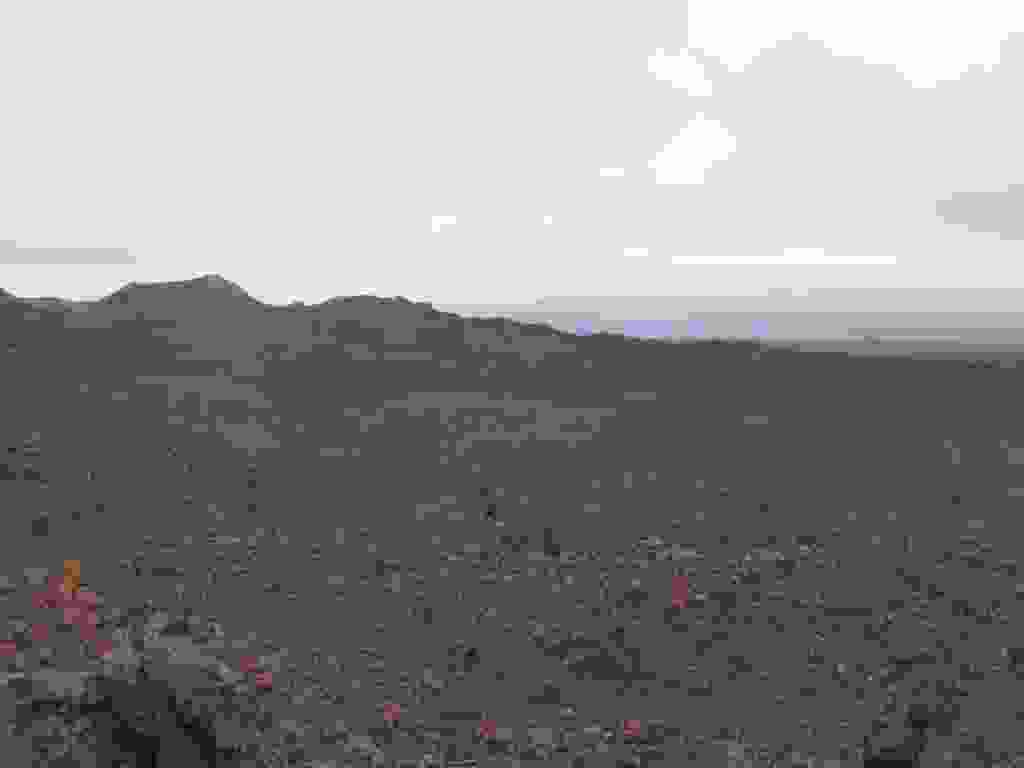
\includegraphics[width=\mywidth]{../wp-content/uploads/2015/07/P7055357-1024x768.jpg} \end{center}
\begin{center} 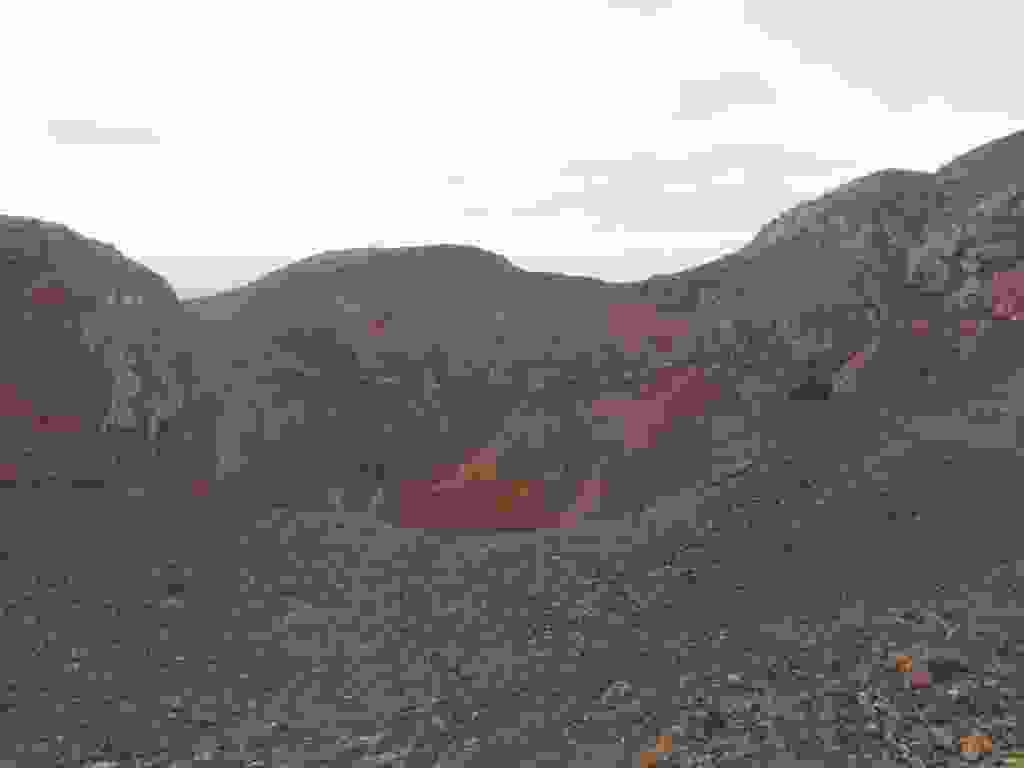
\includegraphics[width=\mywidth]{../wp-content/uploads/2015/07/P7055360-1024x768.jpg} \end{center}
\vspace{-\topsep}
\vspace{-3.25mm}
\pagebreak
~
\begin{center} 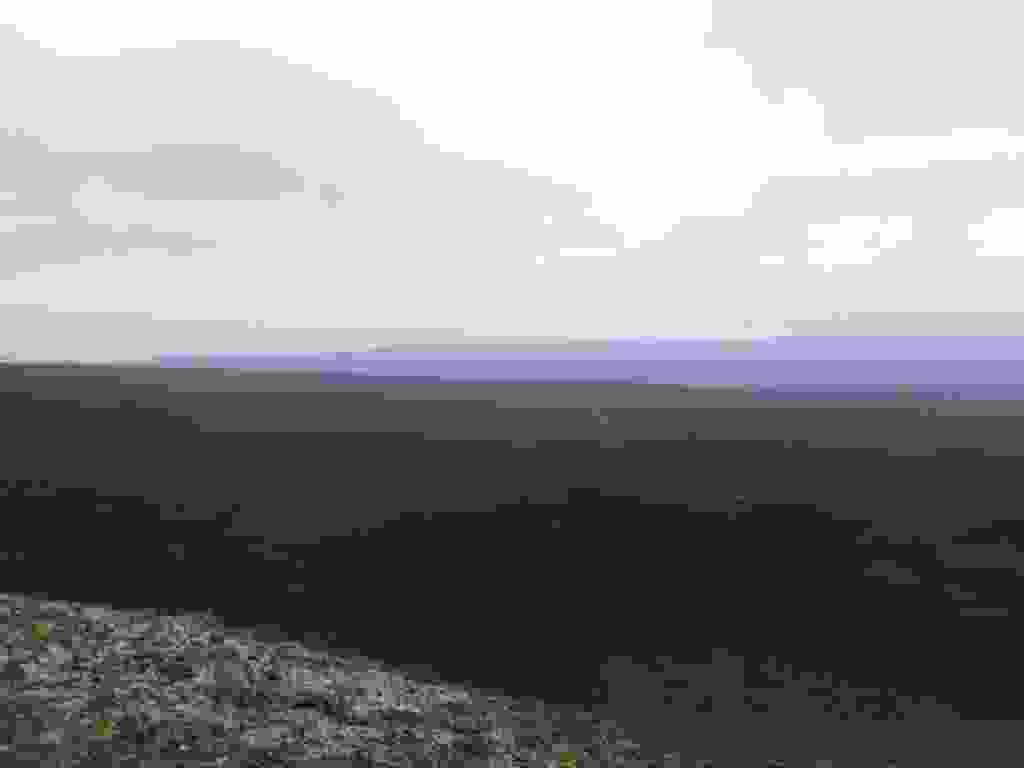
\includegraphics[width=\mywidth]{../wp-content/uploads/2015/07/P7055364-1024x768.jpg} \end{center}
\begin{center} 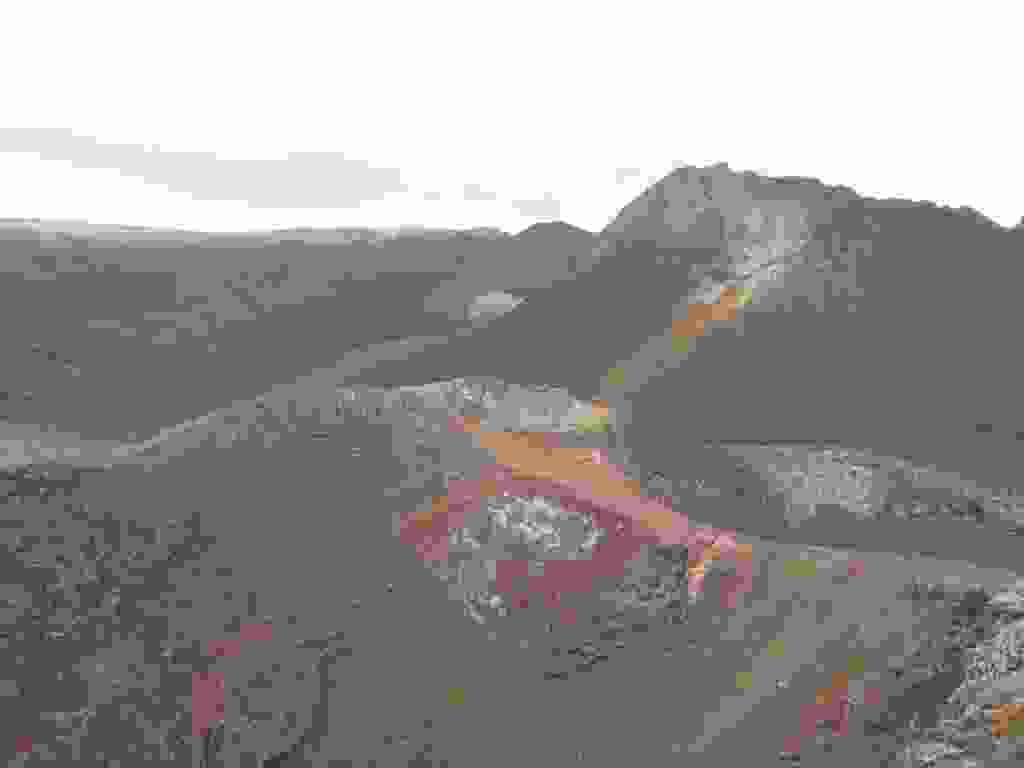
\includegraphics[width=\mywidth]{../wp-content/uploads/2015/07/P7055366-1024x768.jpg} \end{center}
\vspace{-\topsep}
\vspace{-3.25mm}
\pagebreak

Je fais le tour de snorkeling de Los Tuneles à 1h de bateau de la ville. \\
\begin{center} 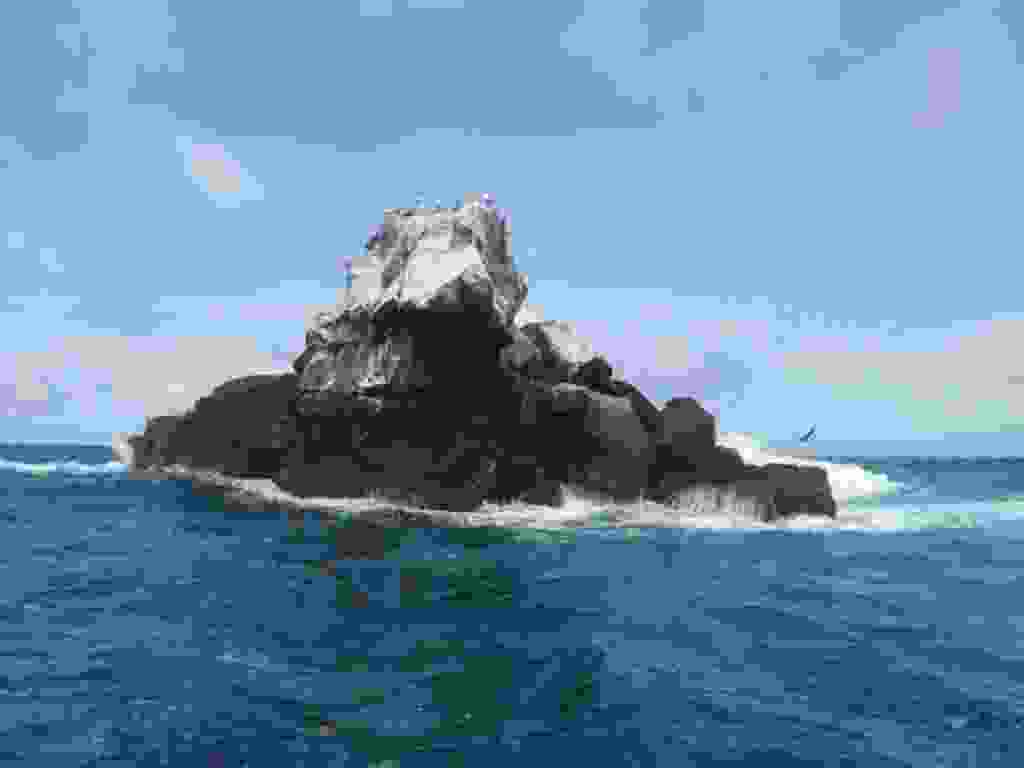
\includegraphics[width=\mywidth]{../wp-content/uploads/2015/07/P7065372-1024x768.jpg} \end{center}

Sur le trajet on descend du bateau pour observer des raies manta : vraiment impressionnantes. 
Les pingouins des Galapagos: 
\begin{center} \includegraphics[width=\mywidth]{../wp-content/uploads/2015/07/P7065376-1024x768.jpg} \end{center}
\vspace{-\topsep}
\pagebreak

Puis 2 snorkeling où l'on peut voir beaucoup de poissons, des tortues marines, des requins (qui dorment), des hippocampes. 
\begin{center} \includegraphics[width=\mywidth]{../wp-content/uploads/2015/07/P7065381-1024x768.jpg} \end{center}
~\\
\begin{center} \includegraphics[width=\mywidth]{../wp-content/uploads/2015/07/P7065384-1024x768.jpg} \end{center}
\vspace{-\topsep}
\pagebreak

J'ai voulu prendre des photos avec l'appareil étanche : il a pris l'eau et ne marche plus ! Heureusement que c'est arrivé à la fin des Galapagos !
\vfill
Enfin il fallait bien gouter un bon poisson des Galapagos. 
\vfill
\begin{center} \includegraphics[width=\mywidth]{../wp-content/uploads/2015/07/P7035246-1024x768.jpg} \end{center}
\vfill
Accompagné d'une bière équatorienne il est bien passé ! 
\vfill
\begin{center} \includegraphics[width=\mywidth]{../wp-content/uploads/2015/07/P7035244-1024x768.jpg} \end{center}
\vspace{-\topsep}
\vspace{-0.75mm}
